\documentclass[12pt]{article}
\title{\textbf{TELLIE PCA: \\ Processing automation}}
\date{February 2023}
\author{Michal Rigan}
\usepackage{hyperref}
\hypersetup{
     colorlinks   = true,
     urlcolor = blue,
     citecolor    = grey
}
\hypersetup{colorlinks=true}
\usepackage{graphicx}
\usepackage{listings}
\lstset{
    basicstyle=\ttfamily\footnotesize,
    frame=single, % adds a frame around the code
    xleftmargin=3.4pt,
    xrightmargin=3.4pt,
}
\graphicspath{ {images/} }
\begin{document}

\maketitle{}

\vspace{7cm}
\paragraph{}
This document describes what the TELLIE PCA automation does, why, and how.
\clearpage

\tableofcontents

\clearpage

\section{Content}
\paragraph{}
\begin{itemize}
	\item Why automation
	\item Overview
	\item Data-taking
	\begin{itemize}
		\item Validation \#1
	\end{itemize}
	\item Data-processing
	\begin{itemize}
		\item PCA table generation
		\begin{itemize}
			\item Beamspot fit
			\item Direction fit
			\item Angular systematic
			\item Injection time fit
		\end{itemize}
		\item Validation \#2
		\item PCA constants
		\item Benchmarking
		\item Monitoring
	\end{itemize}
	\item Code %mention checks, structure
	\item Deploying %(mention requirements here: rat, python, dbs...)
	\item Running
	\item ToDos
	\item Other documentation %tellie guides (2), PCA guide, my thesis
\end{itemize}

\section{Why automation}
\paragraph{}
The process of extracting and validating PCA constants from TELLIE data is complex. This piece of software was developed to streamline the process of obtaining the PCA constants, at reasonably high speed. \\
Additionally, it was designed to:
\begin{itemize}
	\item be independent of the method used for Data-taking
	\item be modular, easily modifiable and configurable
	\item require minimal human input
	\item provide monitoring
	\item be mostly standalone
\end{itemize}

\section{Overview}
\paragraph{}
The TELLIE PCA Automation overview is shown in Figure~\ref{fig:overview}.\\There are two main parts: TELLIE \textbf{\texttt{Data-taking}} and \textbf{\texttt{Data-processing}}.

\paragraph{}
Data-taking is done independently of the processing (as the exact method was not yet finalised before developing processing). More information can be found in \href{https://www.snolab.ca/snoplus/private/DocDB/cgi/ShowDocument?docid=7612}{TELLIE Data-taking automation document}. It should be noted that \texttt{Validation \#1} is taken care of by Data-processing.

\paragraph{}
Data-processing is everything that is done with TELLIE PCA data once it is stored. This includes performing checks on the data, making fits required for further processing, generating tables (both local and online), extracting PCA constants, benchmarking these constants, and a suite of monitoring for these steps. These will be described below.

\begin{figure}
\centering
\noindent\makebox[1\textwidth]{
  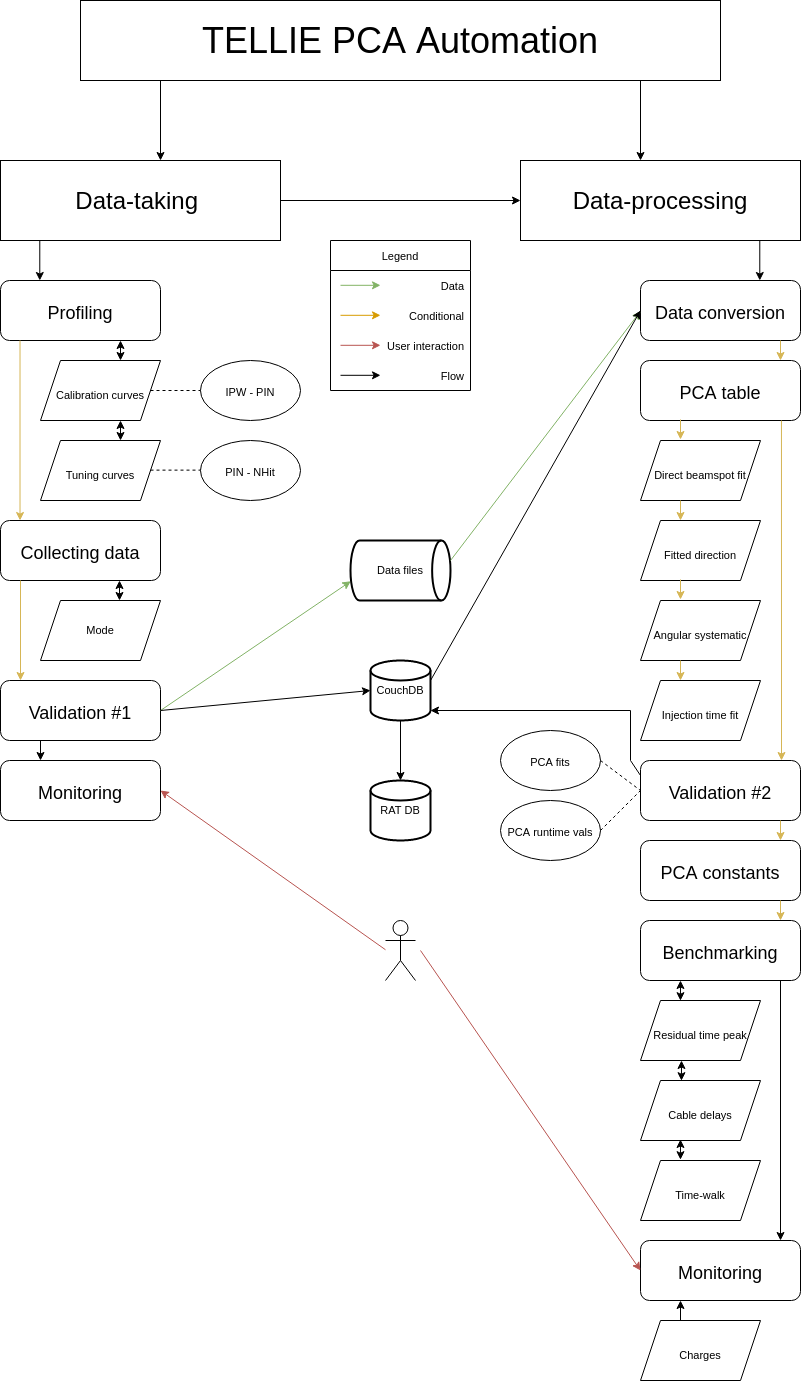
\includegraphics[width=0.9\textwidth]{./plots/overview.png}}
  \caption{\centering Overview of the TELLIE PCA Automation.}
  \label{fig:overview}
\end{figure}

\section{Data-taking}
\subsection{Validation \#1}\label{sec:val1}
\paragraph{}
As mentioned above, even though \texttt{Validation \#1} is logistically part of Data-taking, it is performed by Data-processing, and is also independent of the method used to take data.\\
\textbf{Goal:} Validate that the data is of required quality for PCA.

\paragraph{}
Some of the checks performed are: correct fibre, number of events, number of EXTA events, passed hits, cuts on PMTs, checks on LPC, run lenght, frequency, NHit distribution, NHit over time, delays, time of hits over time, number of peaks, PMTs in beamspot, PMT occupancy, PIN, PIN vs NHit, events over subrruns, and more.

\paragraph{}
The corresponding monitoring page will show basic information for this run; data for events, hits, and times; NHit information; PMTs information; Cuts; Flags; and associated plots. The flags are of special importance, as they form a 'bitword'. This bitword is shown in the list page for each fibre for particular dataset.\\
Examples from the monitoring are shown in Figures~\ref{fig:val1}, \ref{fig:val2}, \ref{fig:val3}, \ref{fig:val4}, \ref{fig:val5}, \ref{fig:val6}, \ref{fig:val7}, \ref{fig:val8}, \ref{fig:val9}, \ref{fig:val10}, \ref{fig:val11}, \ref{fig:val12}, \ref{fig:val13}, \ref{fig:val14}, and \ref{fig:val15}.

\begin{figure}
\centering
\noindent\makebox[1\textwidth]{
  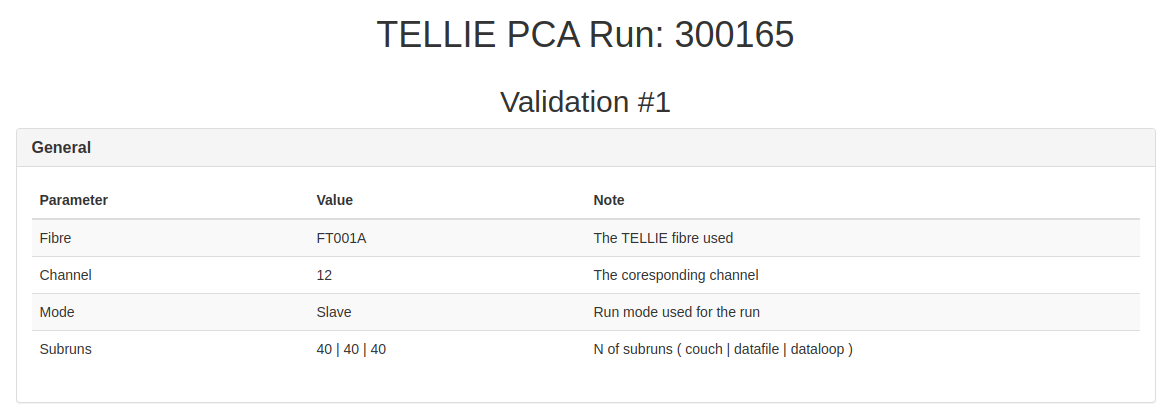
\includegraphics[width=1.1\textwidth]{./plots/val1.png}}
  \caption{\centering \texttt{Validation \#1}: General information.\hspace{\textwidth}This is useful to confirm that the expected fibre is being used, the mode of firing is correct, and that the number of subruns is consistent.}
  \label{fig:val1}
\end{figure}

\begin{figure}
\centering
\noindent\makebox[1\textwidth]{
  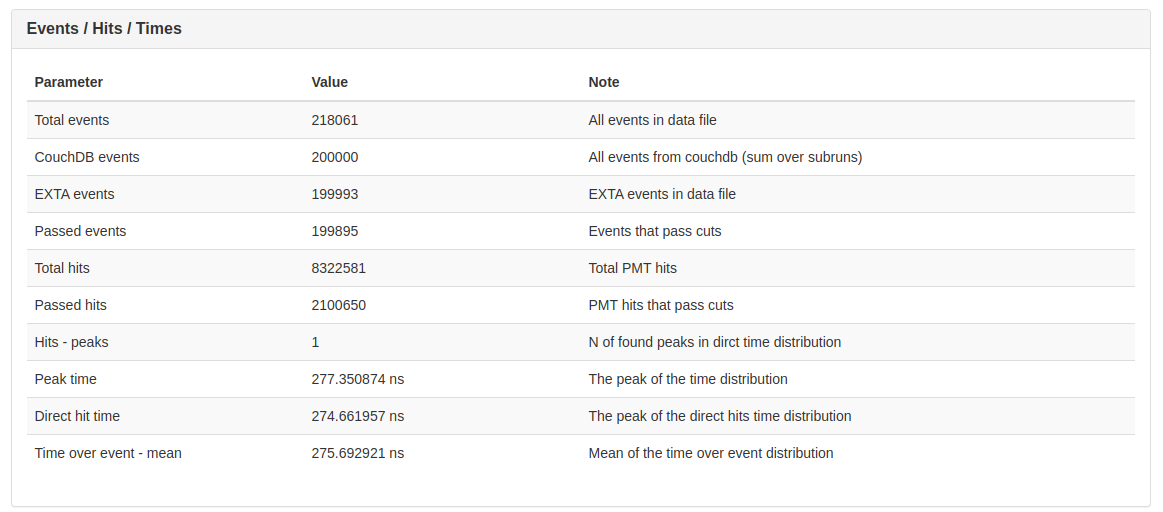
\includegraphics[width=1.1\textwidth]{./plots/val2.png}}
  \caption{\centering \texttt{Validation \#1}: Information regarding events, hits, and times.\hspace{\textwidth}Important features: the number of total events should be equal to or more than CouchDB events. CouchDB events should correspond to the number of requested TELLIE events. The number of EXTA events should be close to CouchDB events (some will be lost due to stolen triggers). Most events should pass checks. The percentage of passed hits will be always low ($\sim$25\%) mostly due to the angular cut, defining the beamspot. The peak times should all be very similar (within few ns). Finally, the direct hit time should not change (much) over datasets, as long as we are not chaning the environment (scintillator) anymore.}
  \label{fig:val2}
\end{figure}

\begin{figure}
\centering
\noindent\makebox[1\textwidth]{
  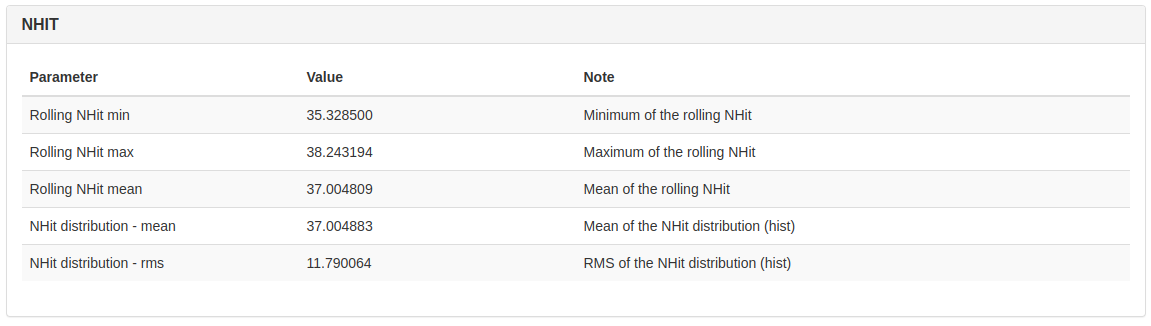
\includegraphics[width=1.1\textwidth]{./plots/val3.png}}
  \caption{\centering \texttt{Validation \#1}: NHit information.\hspace{\textwidth}The NHit should be close to the expected value (this was 40-42 for old datasets). There should only be a small variation.}
  \label{fig:val3}
\end{figure}

\begin{figure}
\centering
\noindent\makebox[1\textwidth]{
  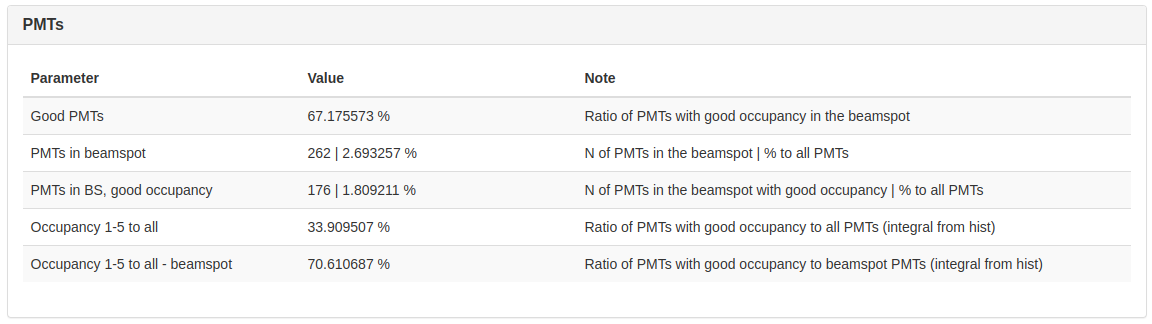
\includegraphics[width=1.1\textwidth]{./plots/val4.png}}
  \caption{\centering \texttt{Validation \#1}: PMT statistics.\hspace{\textwidth}We should make sure we are hitting PMTs in the beamspot, and that these PMTs have good occupancy (between 1-5\%, as to have high enough statistics above noise to extract the constants, but to avoid being contamined by multiple PE hits).}
  \label{fig:val4}
\end{figure}

\begin{figure}
\centering
\noindent\makebox[1\textwidth]{
  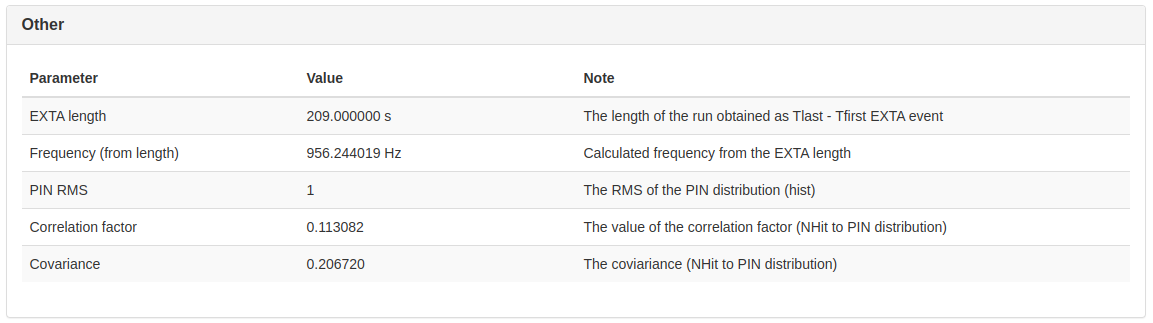
\includegraphics[width=1.1\textwidth]{./plots/val5.png}}
  \caption{\centering \texttt{Validation \#1}: Other information, including calculated run length from EXTA events, calculated frequency, and correlation between PIN and NHit.\hspace{\textwidth}We should check the real run length and frequency are as expected (they will be slightly lower than expected, due to missing EXTA triggers).}
  \label{fig:val5}
\end{figure}

\begin{figure}
\centering
\noindent\makebox[1\textwidth]{
  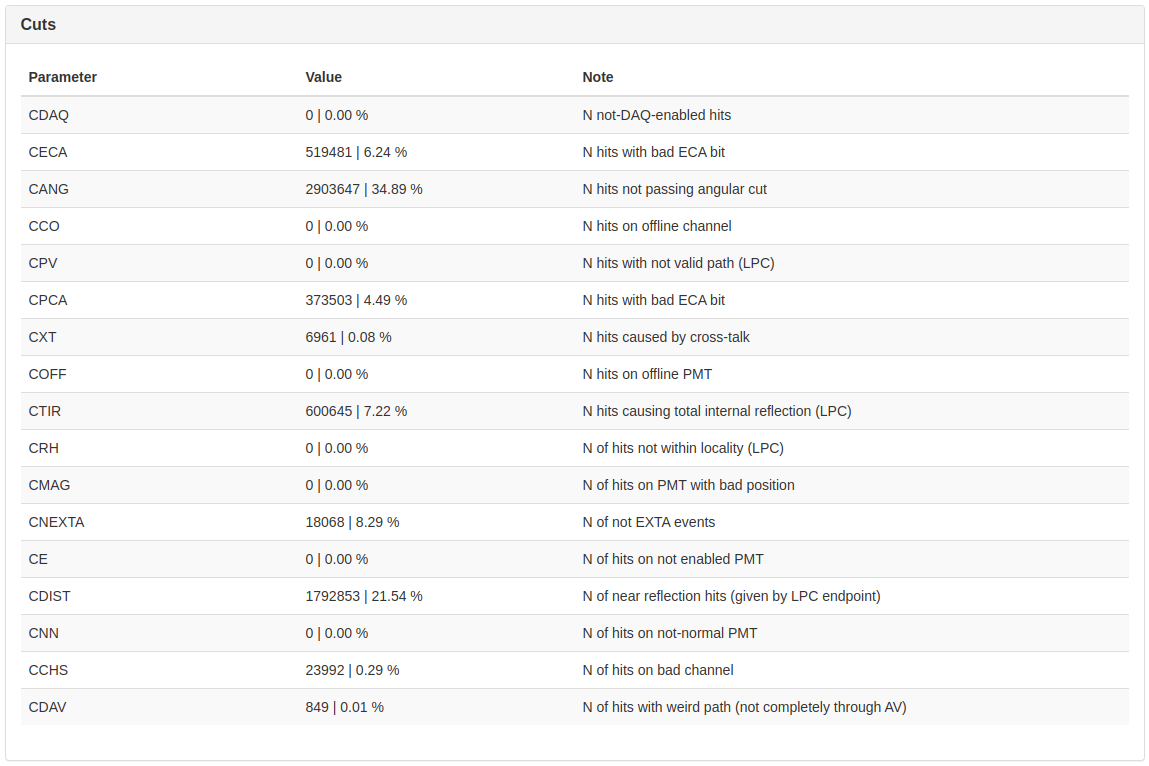
\includegraphics[width=1.1\textwidth]{./plots/val6.png}}
  \caption{\centering \texttt{Validation \#1}: Hit statistics, showing the number of hits that were cut, by category.\hspace{\textwidth}Check cuts on hits and PMTs. Should especially look for outliers. The angular cut will always be big, and that is ok, as we only want to use PMTs in the beamspot (other fibres will cover other PMTs, to get the preferred occupancy).}
  \label{fig:val6}
\end{figure}

\begin{figure}
\centering
\noindent\makebox[1\textwidth]{
  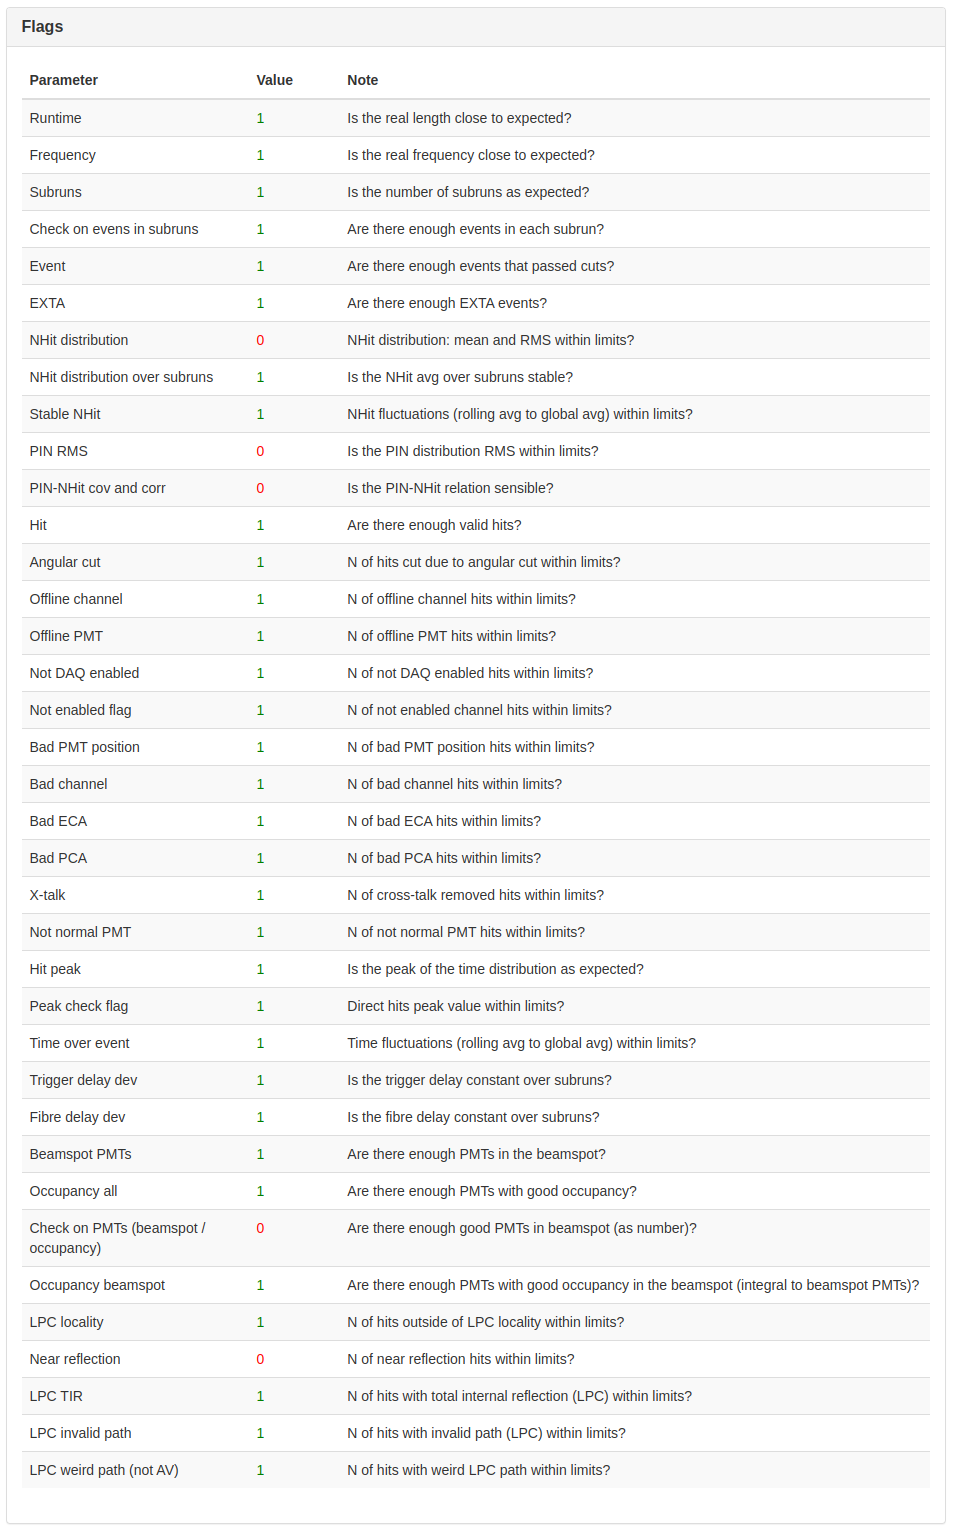
\includegraphics[width=0.85\textwidth]{./plots/val7.png}}
  \caption{\centering \texttt{Validation \#1}: Flags. These are the results of checks/tests on a variety of run/hits atributes. The comments should be a reasonable hint to what each check does.}
  \label{fig:val7}
\end{figure}

\begin{figure}
\centering
\noindent\makebox[1\textwidth]{
  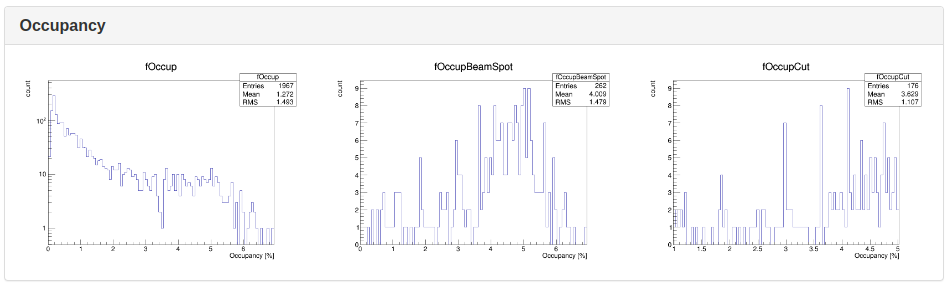
\includegraphics[width=1.1\textwidth]{./plots/val8.png}}
  \caption{\centering \texttt{Validation \#1}: Plots showing occupancy information.\hspace{\textwidth}We should make sure that there are enough PMTs in the beamspot with the required occupancy ($>$100).}
  \label{fig:val8}
\end{figure}

\begin{figure}
\centering
\noindent\makebox[1\textwidth]{
  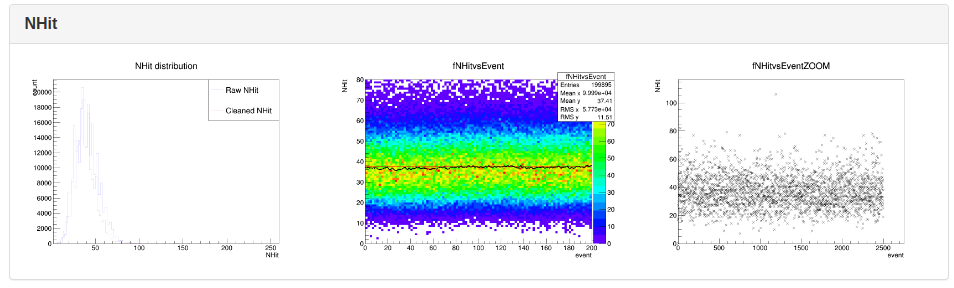
\includegraphics[width=1.1\textwidth]{./plots/val9.png}}
  \caption{\centering \texttt{Validation \#1}: Plots showing NHit information.\hspace{\textwidth}The NHit distribution should be approximately gaussian, with the peak around the expected value (40-42). The NHit should be stable over time, and there should be no noticeable drop at the start of the run.}
  \label{fig:val9}
\end{figure}

\begin{figure}
\centering
\noindent\makebox[1\textwidth]{
  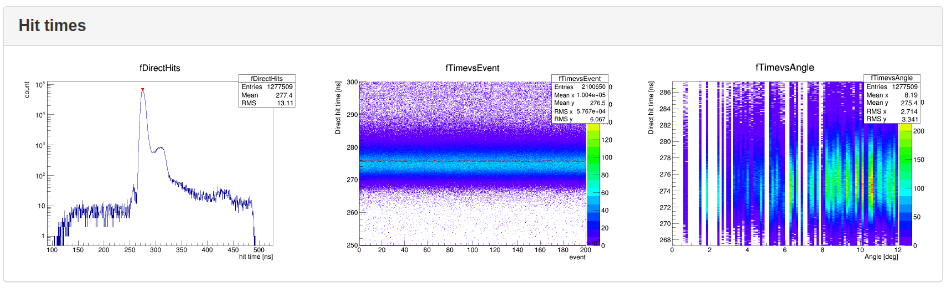
\includegraphics[width=1.1\textwidth]{./plots/val10.png}}
  \caption{\centering \texttt{Validation \#1}: Plots showing hit times information.\hspace{\textwidth}Similar to NHit, we should confirm the peak is around expected value, the times are consistend over events, and there is no high variation with angle.}
  \label{fig:val10}
\end{figure}

\begin{figure}
\centering
\noindent\makebox[1\textwidth]{
  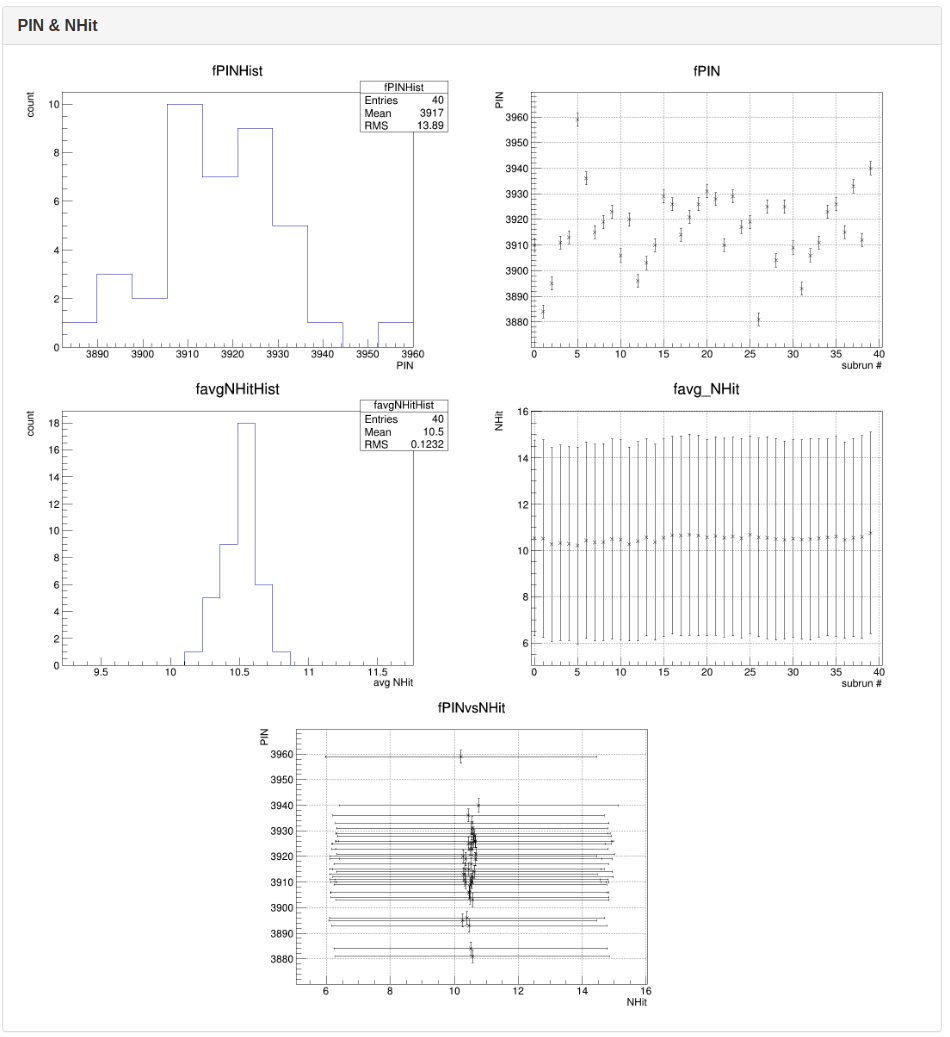
\includegraphics[width=1.1\textwidth]{./plots/val11.png}}
  \caption{\centering \texttt{Validation \#1}: Plots showing PIN and NHit information.\hspace{\textwidth}The PIN values should have low variation (within 100s) and there should be no clear trend over subruns. The NHits here are per subrun, therefore the low value. It should be stable over subruns. Finally, there should be positive correlation between the NHit and PIN (mind the range of erros).}
  \label{fig:val11}
\end{figure}

\begin{figure}
\centering
\noindent\makebox[1\textwidth]{
  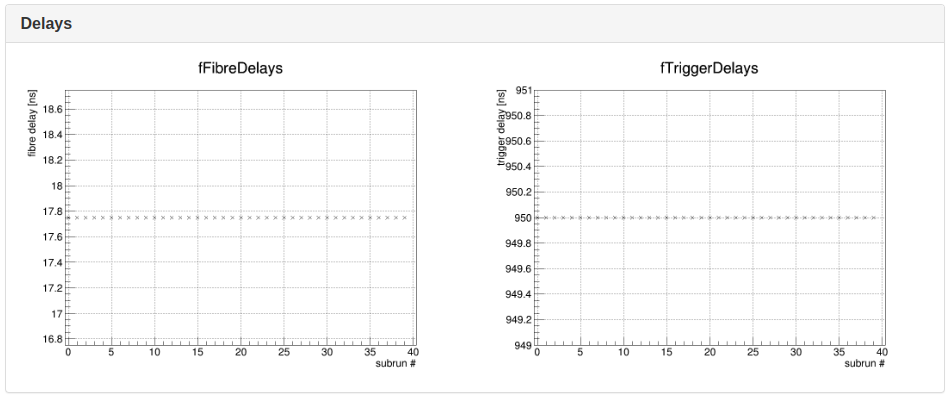
\includegraphics[width=1.1\textwidth]{./plots/val12.png}}
  \caption{\centering \texttt{Validation \#1}: Plots showing delays information.\hspace{\textwidth}Both fibre and trigger delay have to be constant over subruns! Additionally, the trigger delay should be constant across fibres for a dataset. This is essential for the calibration.}
  \label{fig:val12}
\end{figure}

\begin{figure}
\centering
\noindent\makebox[1\textwidth]{
  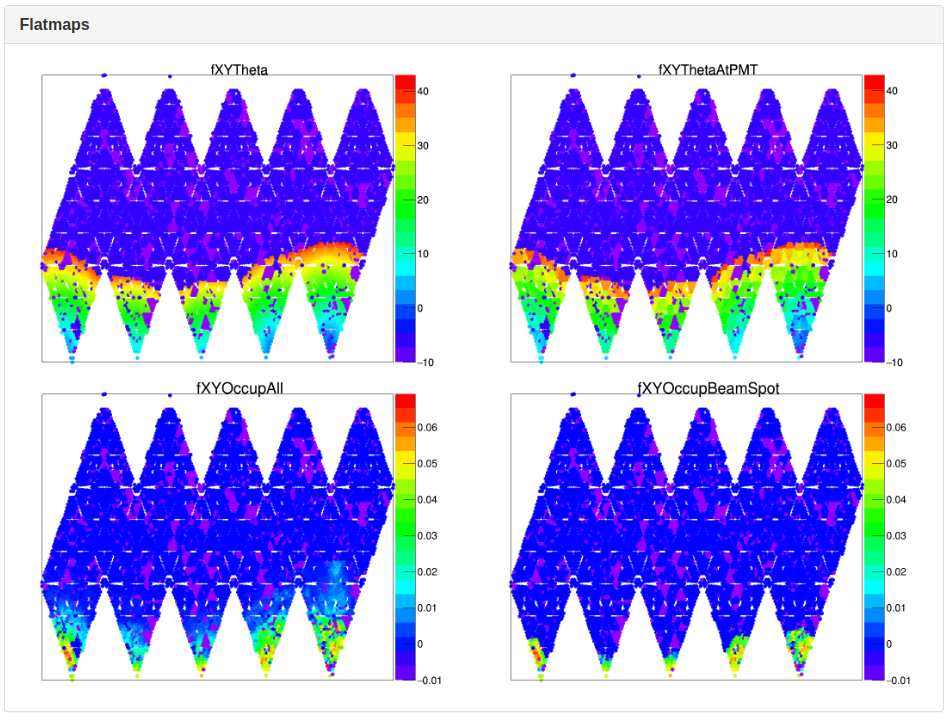
\includegraphics[width=1.1\textwidth]{./plots/val13.png}}
  \caption{\centering \texttt{Validation \#1}: Plots showing data using flatmaps.\hspace{\textwidth}These are to confirm we are getting a beamspot, that the light is there, is not spread out too much, and the occupancy is correct in the beamspot.}
  \label{fig:val13}
\end{figure}

\begin{figure}
\centering
\noindent\makebox[1\textwidth]{
  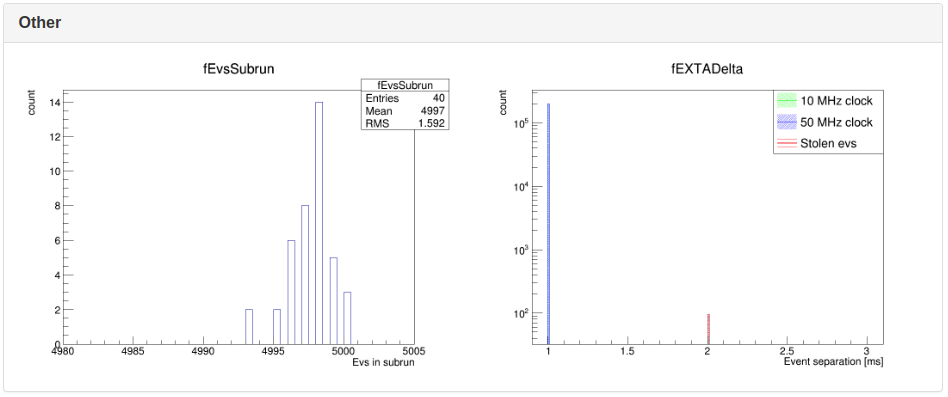
\includegraphics[width=1.1\textwidth]{./plots/val14.png}}
  \caption{\centering \texttt{Validation \#1}: Other information.\hspace{\textwidth}The number of events should be approximately constant over subruns (again, we lose some due to stolen triggers.}
  \label{fig:val14}
\end{figure}

\begin{figure}
\centering
\noindent\makebox[1\textwidth]{
  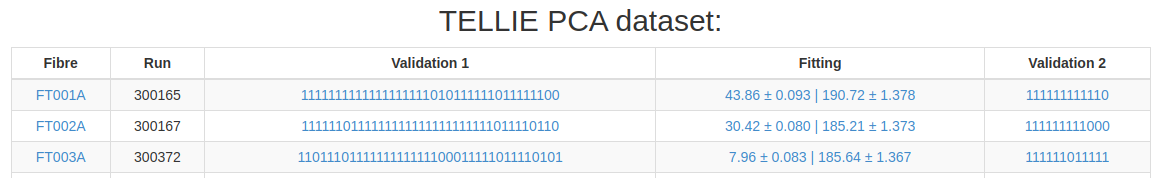
\includegraphics[width=1.1\textwidth]{./plots/val15.png}}
  \caption{\centering \texttt{Validation \#1}: The bitword from \texttt{Validation \#1} shown on the dataset list page for selection of runs.\hspace{\textwidth}The bitword here is made up from the values of flags, corresponding to the checks, for each fibre. Clicking this bitword leads to the \texttt{Validation \#1} page for this run.}
  \label{fig:val15}
\end{figure}

\paragraph{}
The code running \texttt{Validation \#1} is located at:
\begin{lstlisting}
Automation/Processing/validate/TestUser.cc
\end{lstlisting}
This includes the logic for the checks, and generates the bitword. Plots are also made here.

\clearpage

\section{Data-processing}
\subsection{PCA table generation}\label{sec:fits}
\paragraph{}
There are several corrections that need to be fitted for, which are later used for the extraction of PCA constants. The fits need to happen in succession, as the output of one feeds into the next. Between steps, these are stored as text files. After all fits are made, a local table is produced, combining the corrections. This table is loaded by the PCA Processor.\\
\textbf{Goal:} Make fits, obtain corrections required for the extraction of PCA constants. Produce final PCA table.

\subsubsection{Fit: beamspot}

\subsubsection{Fit: direction}

\subsubsection{Fit: angular systematic}

\subsubsection{Fit: Injection time}

\subsection{Validation \#2}\label{sec:val2}
\paragraph{}
Similar to \texttt{Validation \#1}, \texttt{Validation \#2} runs checks on data. In this case, it loads the corrections from the PCA table including the fits.\\
\textbf{Goal:} Check and confirm that the fits are sensible.

\paragraph{}
Some of the tests included here are: mean, rms, min, and max for each correction; distribution, peak(s), and angular dependence for  the residual times; specific trends, and more. 

\begin{figure}
\centering
\noindent\makebox[1\textwidth]{
  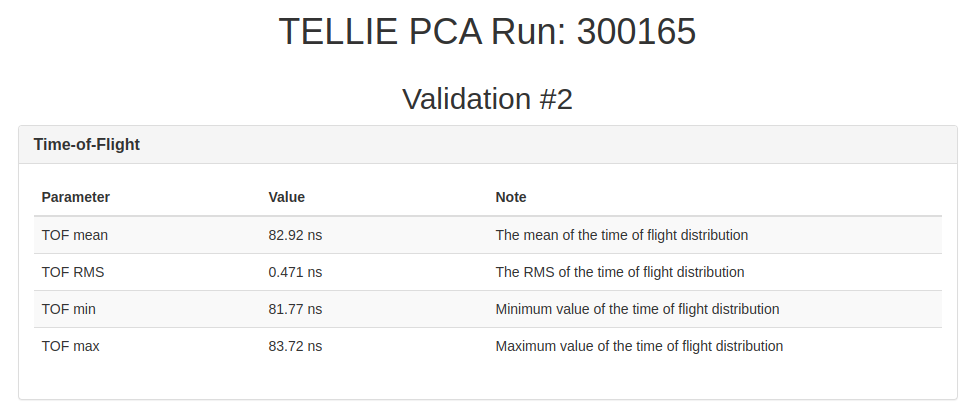
\includegraphics[width=1.1\textwidth]{./plots/val20.png}}
  \caption{\centering \texttt{Validation \#2}: Information relating to Time-of-Flight.\hspace{\textwidth}The mean should always be physical, and the RMS should not be very high ($>$0.5 ns).}
  \label{fig:val20}
\end{figure}

\begin{figure}
\centering
\noindent\makebox[1\textwidth]{
  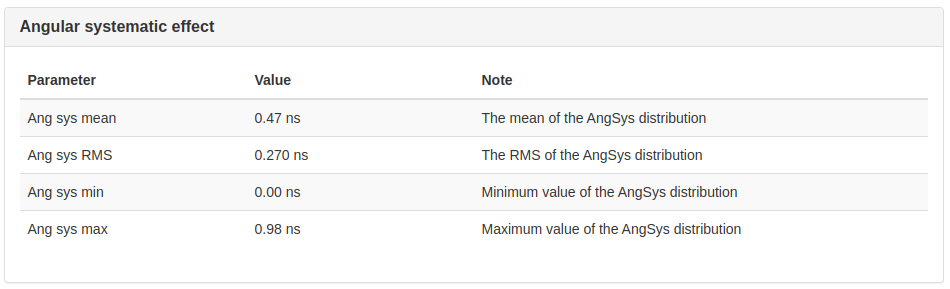
\includegraphics[width=1.1\textwidth]{./plots/val21.png}}
  \caption{\centering \texttt{Validation \#2}: Information relating to angular systematic fit.\hspace{\textwidth}The mean should never be too high ($>$2 ns).}
  \label{fig:val21}
\end{figure}

\begin{figure}
\centering
\noindent\makebox[1\textwidth]{
  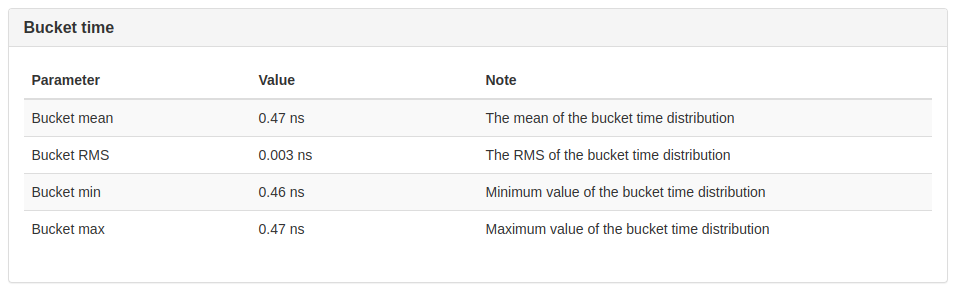
\includegraphics[width=1.1\textwidth]{./plots/val22.png}}
  \caption{\centering \texttt{Validation \#2}: Information relating to bucket time.\hspace{\textwidth}The mean should always be (almost) constant ($\sim$0.47 ns) with low RMS. }
  \label{fig:val22}
\end{figure}

\begin{figure}
\centering
\noindent\makebox[1\textwidth]{
  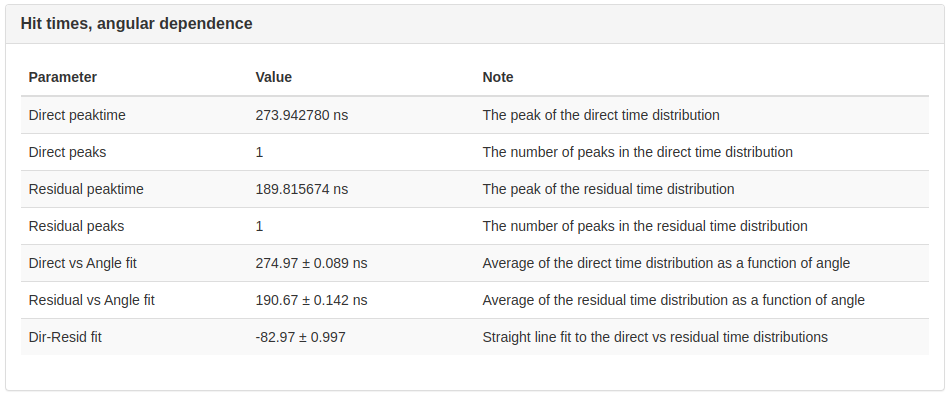
\includegraphics[width=1.1\textwidth]{./plots/val23.png}}
  \caption{\centering \texttt{Validation \#2}: Direct and residual hit times.\hspace{\textwidth}There should only be 1 peak for each distribution, and the peak times should be where expected. A straigh line is expected. }
  \label{fig:val23}
\end{figure}

\begin{figure}
\centering
\noindent\makebox[1\textwidth]{
  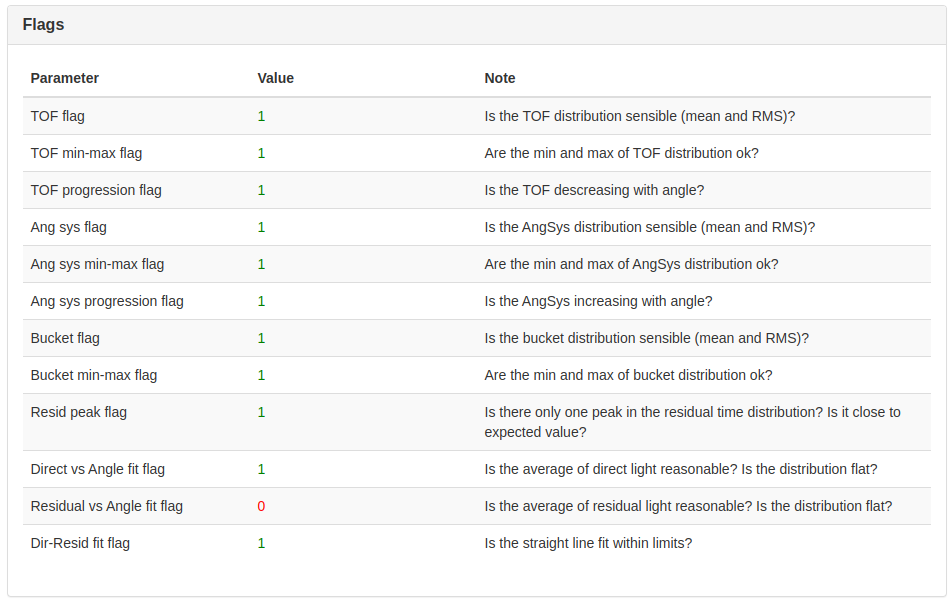
\includegraphics[width=1.1\textwidth]{./plots/val24.png}}
  \caption{\centering \texttt{Validation \#2}: Flags. These are the results of checks/tests on a variety of run/hits atributes. The comments should be a reasonable hint to what each check does.}
  \label{fig:val24}
\end{figure}

\begin{figure}
\centering
\noindent\makebox[1\textwidth]{
  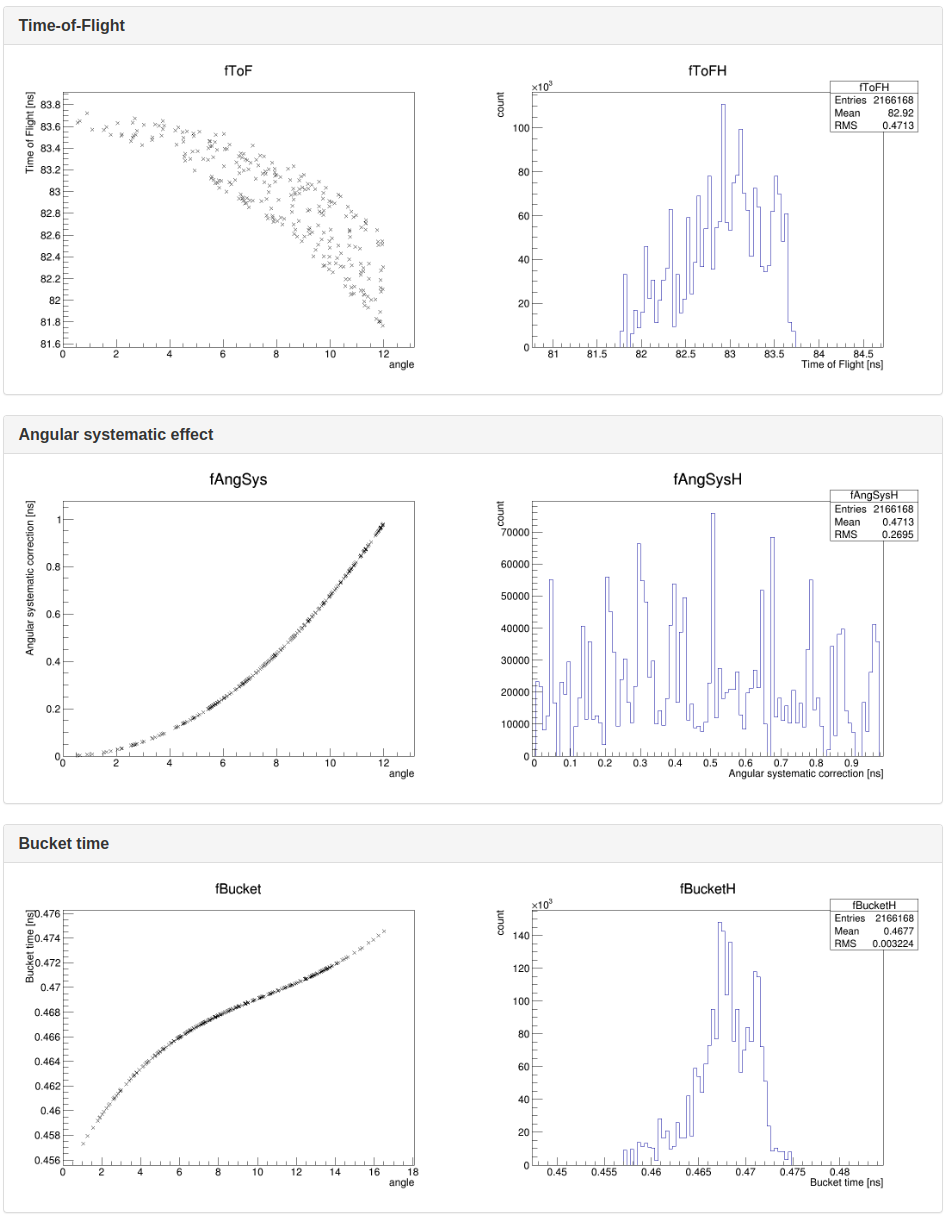
\includegraphics[width=1.1\textwidth]{./plots/val25.png}}
  \caption{\centering \texttt{Validation \#2}: Plots showing the distribution of the corrections.\hspace{\textwidth}ToF should be decreasing over angle, peaking around 83~ns and can never be more than 84~ns. The angular systematic correction has to be increasing with the angle. Bucket time should be a narrow distribution around 0.47~ns. }
  \label{fig:val25}
\end{figure}

\begin{figure}
\centering
\noindent\makebox[1\textwidth]{
  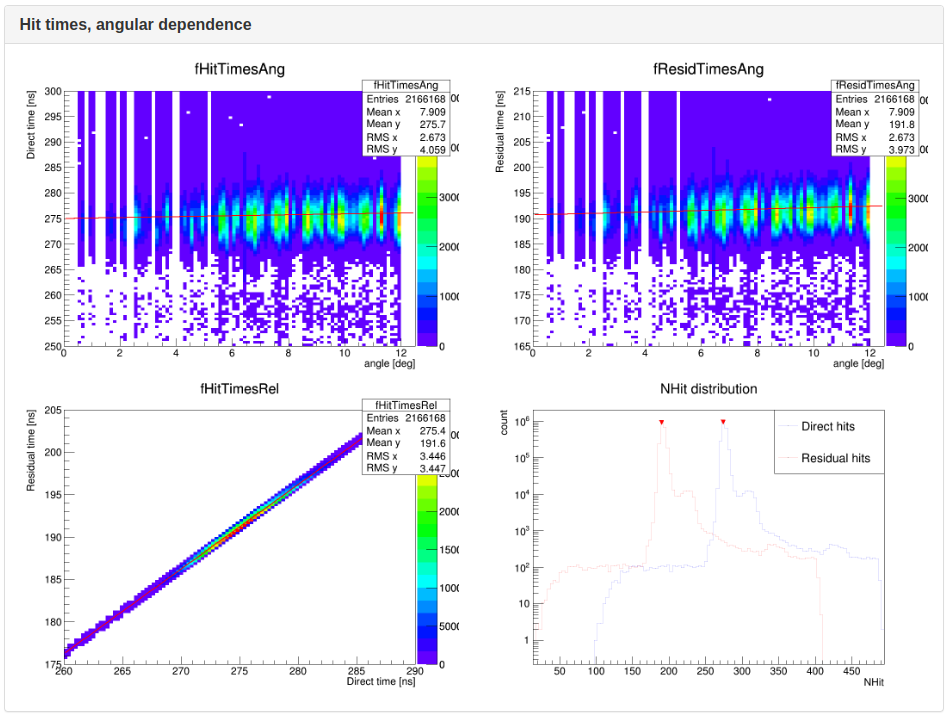
\includegraphics[width=1.1\textwidth]{./plots/val26.png}}
  \caption{\centering \texttt{Validation \#2}: Plots showing the angular dependence of hit times, both raw and residual.\hspace{\textwidth}After corrections, the hit times should be mostly independent of the angle. }
  \label{fig:val26}
\end{figure}

\paragraph{}
The corresponding monitoring page will show the fits information for this run, including Flags; and associated plots. The flags are of special importance, as they form a 'bitword'. This bitword is shown in the list page for each fibre for particular dataset.\\
Examples from the monitoring are shown in Figures~\ref{fig:val20}, \ref{fig:val21}, \ref{fig:val22}, \ref{fig:val23}, \ref{fig:val24}, and \ref{fig:val25}.

\paragraph{}
The code running \texttt{Validation \#2} is located at:
\begin{lstlisting}
Automation/Processing/validate2/TestUser.cc
\end{lstlisting}
This includes the logic for the checks, and generates the bitword. Plots are also made here.

\clearpage

\subsection{Comparing PCA tables}
\textbf{Goal:} Compare the PCA tables (including corrections) for neighbouring datasets. This is useful to monitor stability of the system and to highlight outliers.

\subsection{PCA constants}
\textbf{Goal:} Run the PCA Processor that extract the pca constants (both timing and charge).

\subsection{Benchmarking}
\paragraph{}
This process is used to actually load, use, and compare the PCA constants - cable delays, time-walk fit, and charge fits: threshold, peak, hhp for QHS and QHL.\\
\textbf{Goal:} Compare the set of constants against the closest (previous) set. Useful to see overall stability and for highlighting outliers.

\subsection{Monitoring}
\paragraph{}
This is the most important part for the user. Every step of the system creates logs and plots that are available online on Minard. There are many pages, and everything important (and more) is presented. 
\textbf{Goal:} Provide monitoring of each step of the chain. Also compares fibres and PMTs between datasets.

\paragraph{}
Most parts of the system will be highlighted here. A good rule to using minard portion of the TELLIE PCA processing is that most things are clickable and will lead to detailed page with logs and plots.

\subsubsection{Where}
\paragraph{}
The minard page for TELLIE PCA Processing can be accessed using the main header bar, by slecting the \textbf{PMTcal} tab, and clicking the \textbf{PCA Tellie Processing}, as shown in Figure~\ref{fig:min1}.

\begin{figure}
\centering
\noindent\makebox[1\textwidth]{
  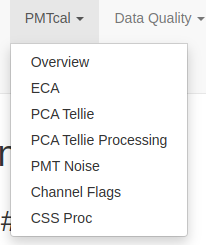
\includegraphics[width=0.4\textwidth]{./plots/min1.png}}
  \caption{\centering \texttt{Minard}: Location of PCA Tellie Processing button.\hspace{\textwidth}This is inside the PMTcal tab.}
  \label{fig:min1}
\end{figure}

\paragraph{}
This leads to the \textbf{TELLIE PCA datasets page}. This is the main/overview page for the TELLIE PCA Processing. It shows the list of datasets (Figure~\ref{fig:min2}), the PMT search box (Figure~\ref{fig:min3}), and the list of thresholds (Figure~\ref{fig:min4}).
\paragraph{}
The list of datasets (Figure~\ref{fig:min2}) is the starting point. Again, most cells are clickable and will lead to more detailed page:
\begin{itemize}
	\item Clicking on the cell in 'Run range' will bring an overview page for that particular dataset, Figure~\ref{fig:min8}.
	\item The 'PCA table' cell will show a page comparing the PCA table associated with that dataset to previous PCA table. Figures~\ref{fig:tab1}, \ref{fig:tab2}, \ref{fig:tab3}, and \ref{fig:tab4}.
	\item 'PCA processor' page shows the results of PCA Processor: Figures~\ref{fig:pca1}, \ref{fig:pca2}, \ref{fig:pca3}, \ref{fig:pca4}, \ref{fig:pca5}, and \ref{fig:pca6}.
	\item 'Benchmarking' shows plot comparing the PCA constants obtained in this dataset to previous constant, shown in Figures~\ref{fig:bench1}, \ref{fig:bench2}, \ref{fig:bench3}, \ref{fig:bench4}, \ref{fig:bench5}, \ref{fig:bench6}, and \ref{fig:bench7}.
	\item 'Status' presents information from parsed log file from PCA Processor. It will list warnings or errors from the PCA processor, Figure~\ref{fig:log0}.
	\item 'TW' shows the time-walk information for this set of constants. PMTs with issues such as too high RMS or high Q tail are listed here. See Figures~\ref{fig:log_tw}, \ref{fig:log1}, \ref{fig:log2}, and \ref{fig:log3}.
	\item 'GF' shows the time-walk information for this set of constants. PMTs with issues such as QHS TH too high or Peakfinder found multiple peaks are listed here. Figures~\ref{fig:log_gf}, \ref{fig:log1}, and \ref{fig:log3}.
	\item Additionally, clicking the 'PCA tables' header lead to page comparing PCA tables across all available datasets. Note Figures~\ref{fig:min5}, \ref{fig:min6}, and \ref{fig:min7}.
	\item It is also possible to look at fibre data across datasets (this is perhaps the most interesting feature). One can get here by clicking the fibre name on the dataset page (Figure~\ref{fig:min8}). A selection of plots are shown in Figure~\ref{fig:min9} and Figure~\ref{fig:min10}.
	\item Finally, there are plots for PMTs for each dataset (Figure~\ref{fig:pmt1} and Figure~\ref{fig:pmt2}) and over datasets (using PMT search, Figure~\ref{fig:min3}).
\end{itemize}

\clearpage

\begin{figure}
\centering
\noindent\makebox[1\textwidth]{
  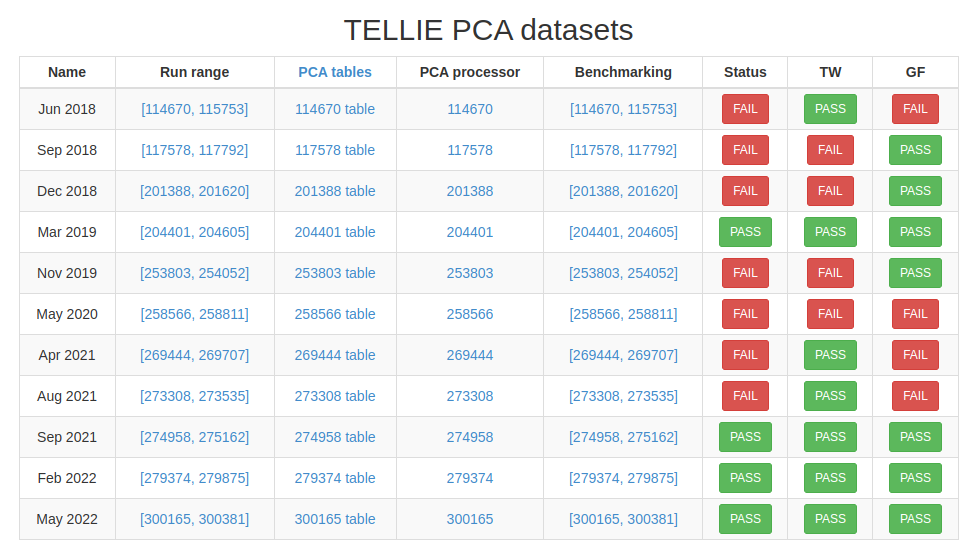
\includegraphics[width=1.1\textwidth]{./plots/min2.png}}
  \caption{\centering \texttt{Minard}: The main table of the main page.\hspace{\textwidth}This table holds a line for each processed dataset. Most cells in here are clickable, leading to a more detailed page or list. These get auto-populated with the processing suite.}
  \label{fig:min2}
\end{figure}

\begin{figure}
\centering
\noindent\makebox[1\textwidth]{
  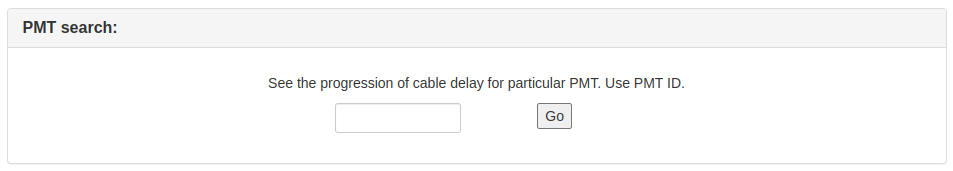
\includegraphics[width=1.1\textwidth]{./plots/min3.png}}
  \caption{\centering \texttt{Minard}: PMT search section.\hspace{\textwidth}One can input a PMT number and a detailed page showing the PMT cable delays over all datasets will be shown.}
  \label{fig:min3}
\end{figure}

\begin{figure}
\centering
\noindent\makebox[1\textwidth]{
  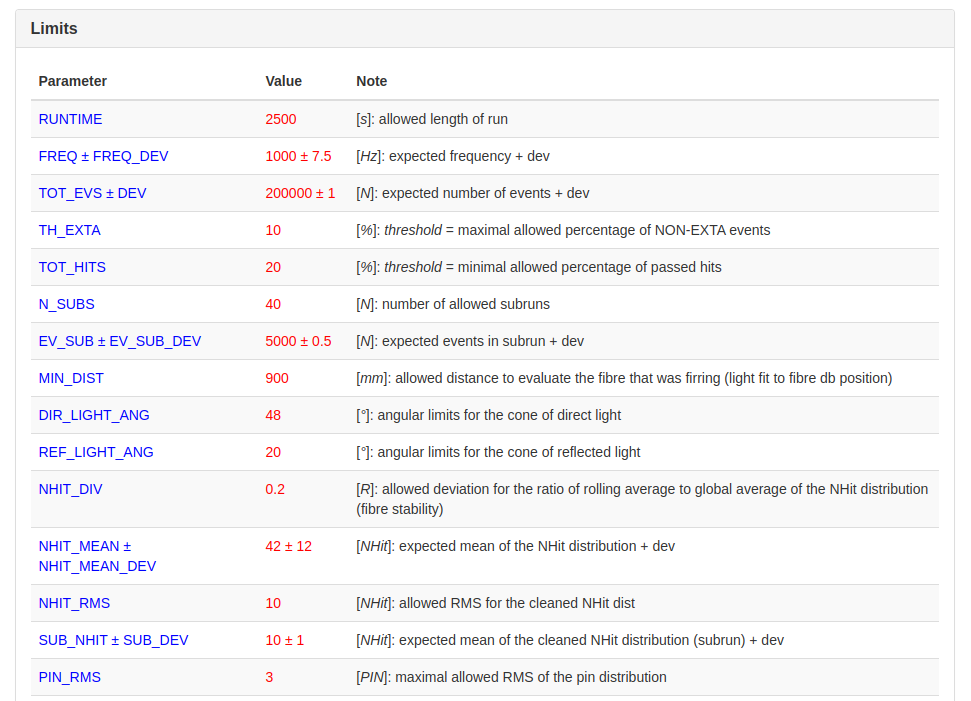
\includegraphics[width=1.1\textwidth]{./plots/min4.png}}
  \caption{\centering \texttt{Minard}: Limits section.\hspace{\textwidth}This section lists the environment thresholds (used for validation checks).}
  \label{fig:min4}
\end{figure}

\begin{figure}
\centering
\noindent\makebox[1\textwidth]{
  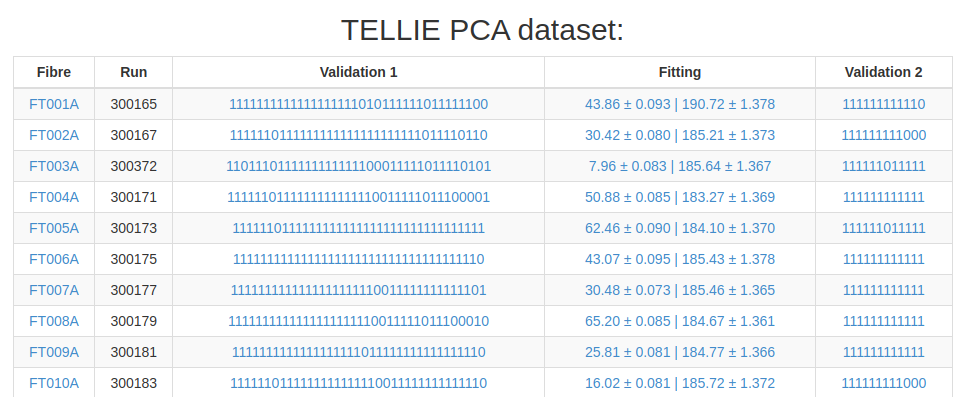
\includegraphics[width=1.1\textwidth]{./plots/min8.png}}
  \caption{\centering \texttt{Minard}: A list for TELLIE PCA dataset.\hspace{\textwidth}. This table shows the bitwords for both validations (see Section~\ref{sec:val1} and Section~\ref{sec:val2}) and results of main fitting parameters (angular b and injection time, see Section~\ref{sec:fits}). Clicking a cell brings up more detailed page with data and plots. One can also click on the fibre name, which shows data for that fibre across all datasets.}
  \label{fig:min8}
\end{figure}

\begin{figure}
\centering
\noindent\makebox[1\textwidth]{
  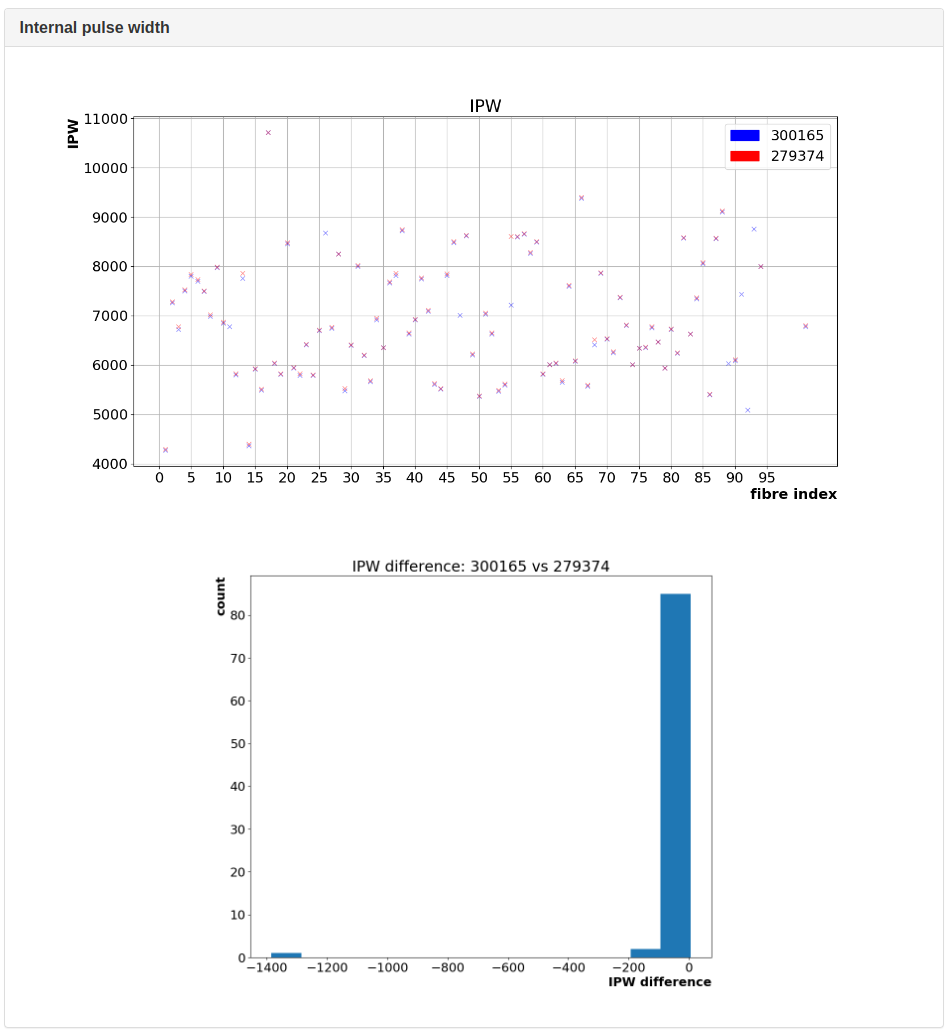
\includegraphics[width=1.1\textwidth]{./plots/tab1.png}}
  \caption{\centering \texttt{Minard}: PCA table for one dataset.\hspace{\textwidth}This serves as a comparison of a single dataset's PCA table to the closest previous dataset's PCA table. These plots: IPW, IPW difference.}
  \label{fig:tab1}
\end{figure}

\begin{figure}
\centering
\noindent\makebox[1\textwidth]{
  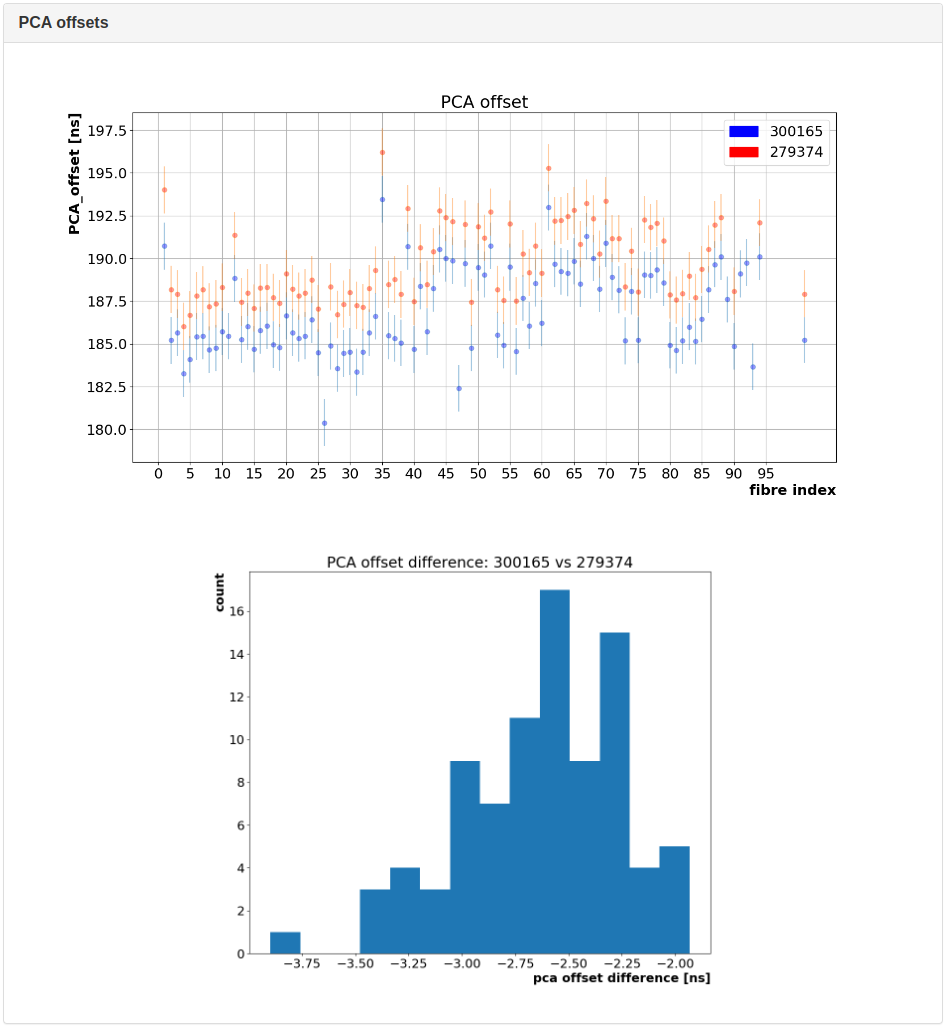
\includegraphics[width=1.1\textwidth]{./plots/tab2.png}}
  \caption{\centering \texttt{Minard}: PCA table for one dataset.\hspace{\textwidth}This serves as a comparison of a single dataset's PCA table to the closest previous dataset's PCA table. These plots: PCA offset (also called injection time), PCA offset difference.}
  \label{fig:tab2}
\end{figure}

\begin{figure}
\centering
\noindent\makebox[1\textwidth]{
  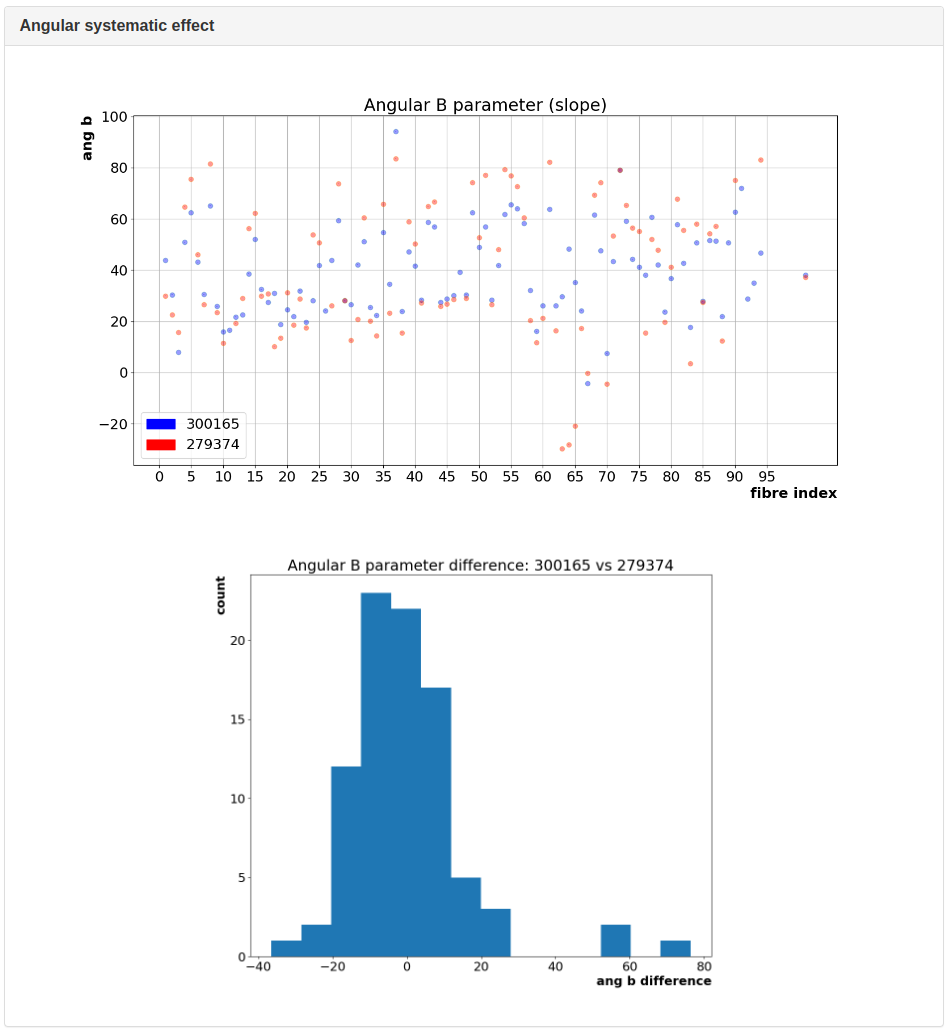
\includegraphics[width=1.1\textwidth]{./plots/tab3.png}}
  \caption{\centering \texttt{Minard}: PCA table for one dataset.\hspace{\textwidth}This serves as a comparison of a single dataset's PCA table to the closest previous dataset's PCA table. These plots: Angular b parameter, angular b parameter difference.}
  \label{fig:tab3}
\end{figure}

\begin{figure}
\centering
\noindent\makebox[1\textwidth]{
  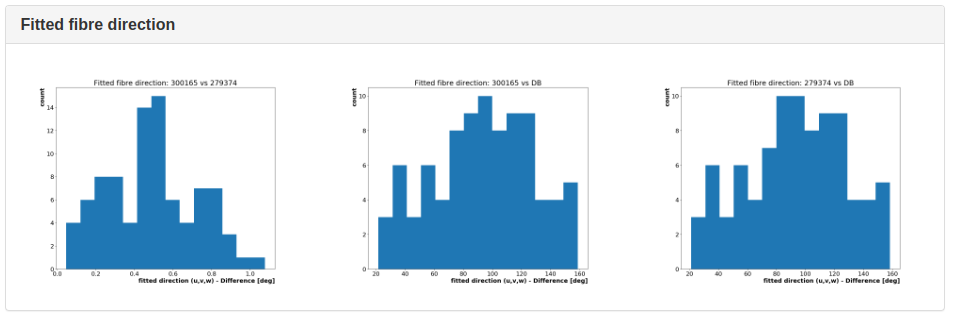
\includegraphics[width=1.1\textwidth]{./plots/tab4.png}}
  \caption{\centering \texttt{Minard}: PCA table for one dataset.\hspace{\textwidth}This serves as a comparison of a single dataset's PCA table to the closest previous dataset's PCA table. These plots: fitted direction.}
  \label{fig:tab4}
\end{figure}

\begin{figure}
\centering
\noindent\makebox[1\textwidth]{
  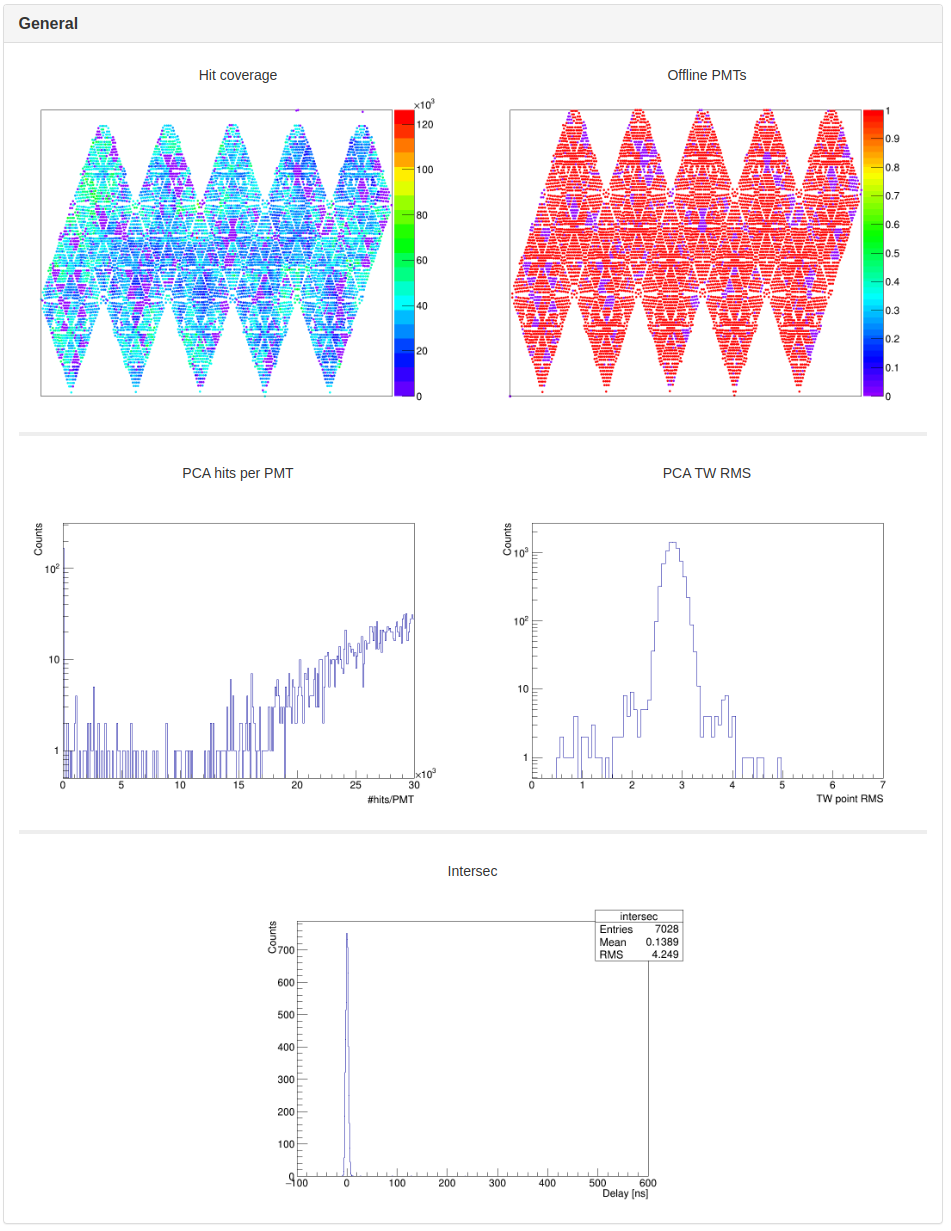
\includegraphics[width=1.1\textwidth]{./plots/pca1.png}}
  \caption{\centering \texttt{PCA Processor}: Hit coverage (hits per PMT), Offline PMTs (purple means offline), PCA hits per PMT (hits passing cuts), PCA TW RMS, PCA intersec.\hspace{\textwidth}}
  \label{fig:pca1}
\end{figure}

\begin{figure}
\centering
\noindent\makebox[1\textwidth]{
  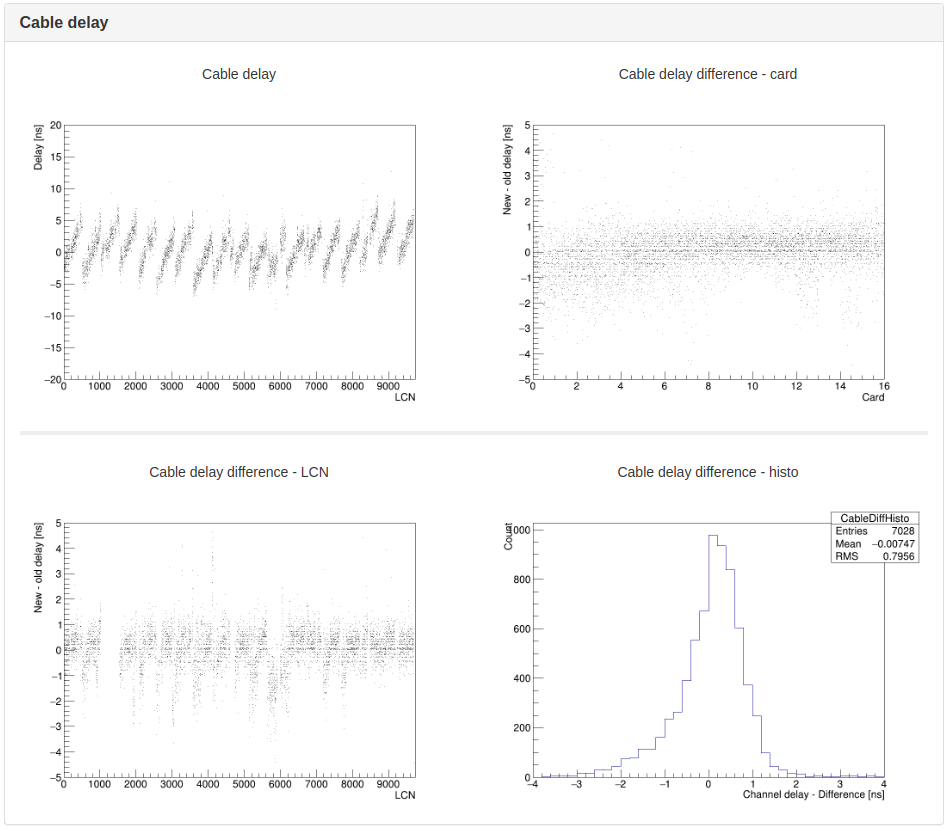
\includegraphics[width=1.1\textwidth]{./plots/pca2.png}}
  \caption{\centering \texttt{PCA Processor}: Cable delays.\hspace{\textwidth}Cable delay per LCN (logical channel number), Cable delays across cards, the difference of this and previous cable delay per LCN, and the difference of this and previous cable delay - histogram. }
  \label{fig:pca2}
\end{figure}

\begin{figure}
\centering
\noindent\makebox[1\textwidth]{
  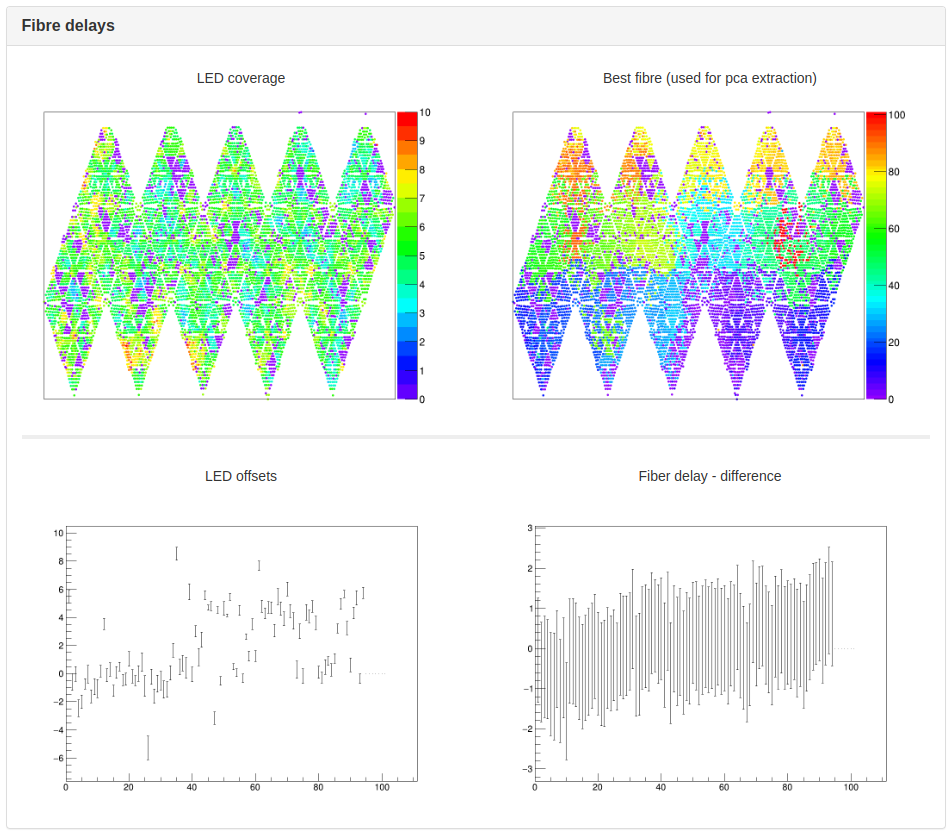
\includegraphics[width=1.1\textwidth]{./plots/pca3.png}}
  \caption{\centering \texttt{PCA Processor}: LED data.\hspace{\textwidth}LED coverage (\# LEDs hitting a PMT), Best fibre (the fibre with highest occupancy (within limits) used for calibration), LED offsets (respective time offset between LEDs), fibre delay (the difference of current and previous LED offset).}
  \label{fig:pca3}
\end{figure}

\begin{figure}
\centering
\noindent\makebox[1\textwidth]{
  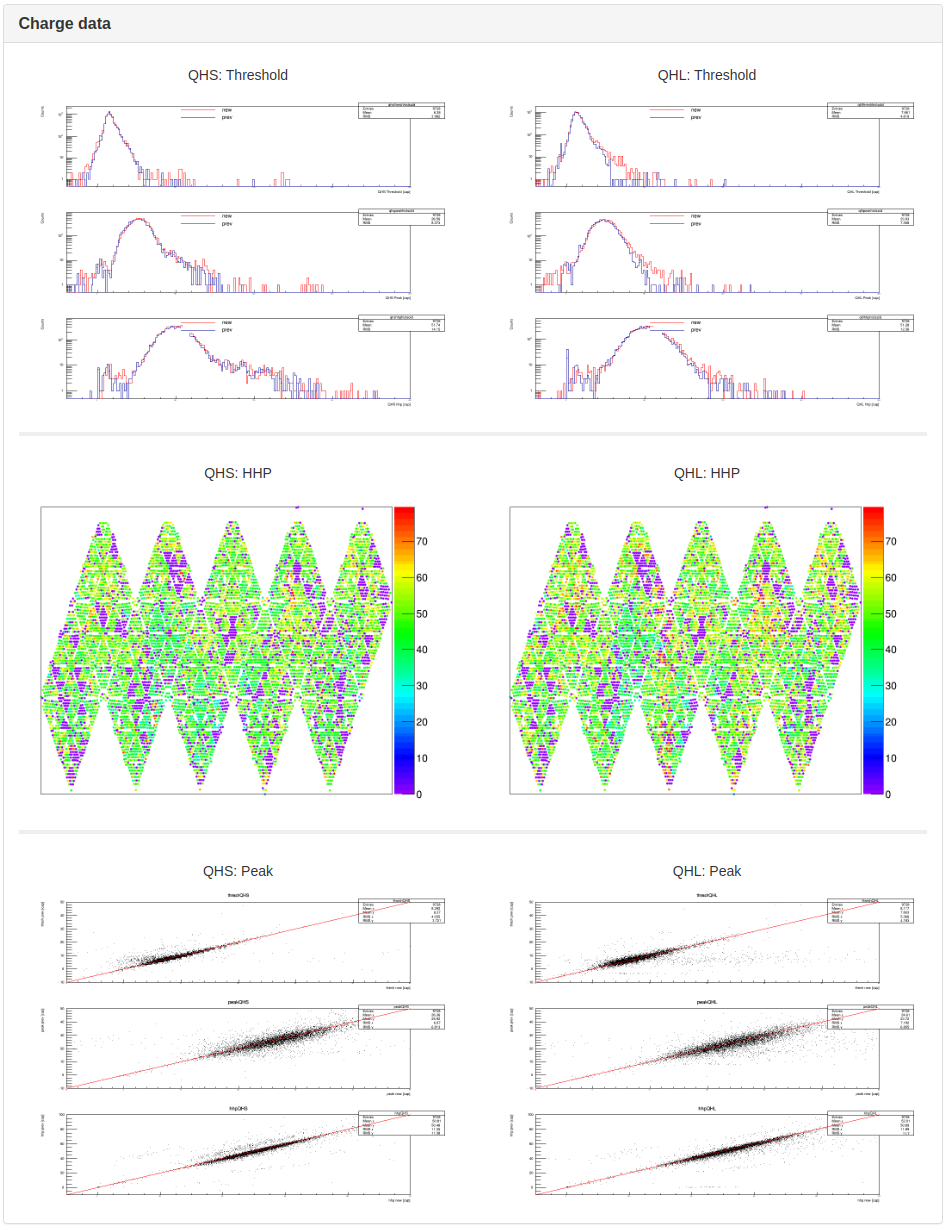
\includegraphics[width=1.1\textwidth]{./plots/pca4.png}}
  \caption{\centering \texttt{PCA Processor}: Charge data.\hspace{\textwidth}The value of threshold, HHP (high half point), and peak for both QHS (left) and QHL (right).}
  \label{fig:pca4}
\end{figure}

\begin{figure}
\centering
\noindent\makebox[1\textwidth]{
  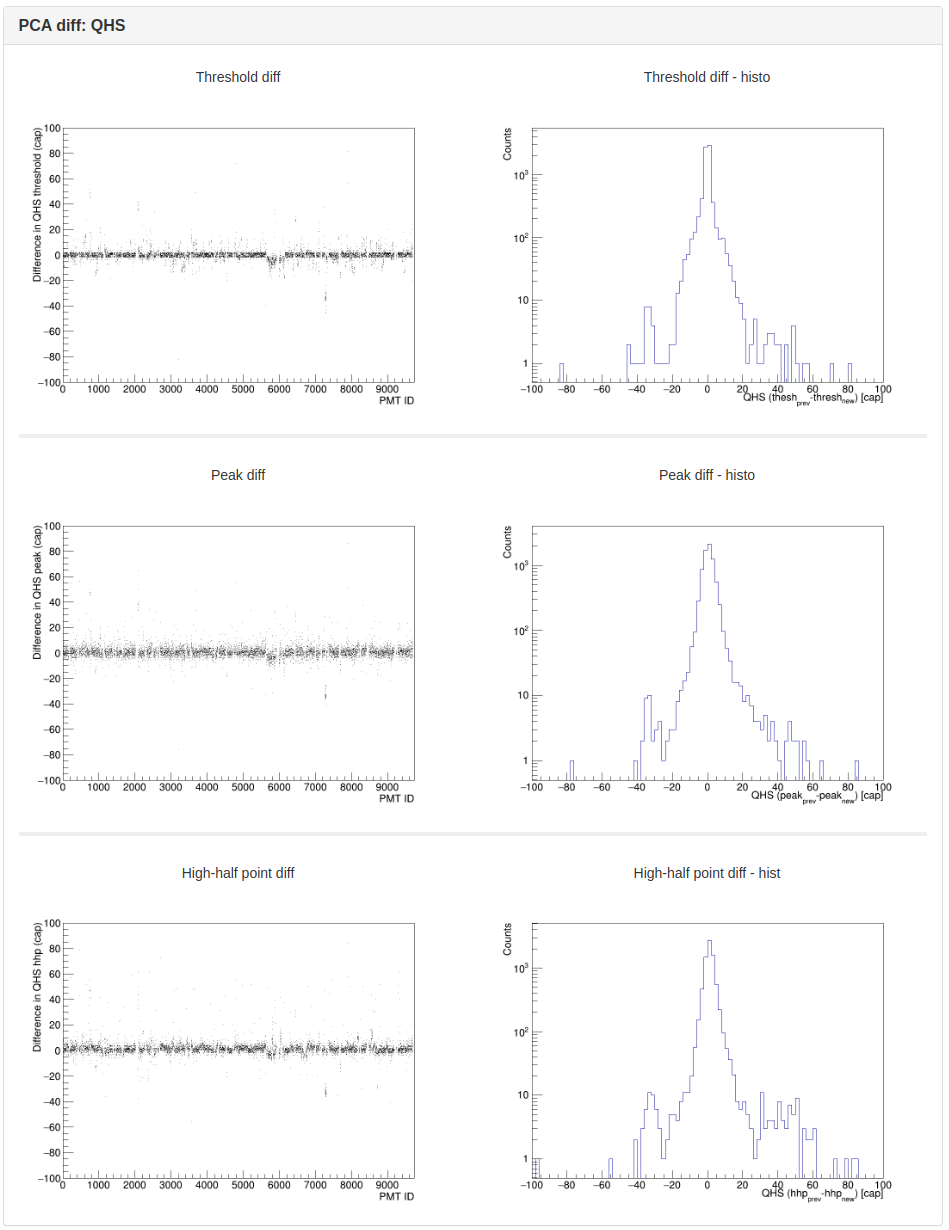
\includegraphics[width=1.1\textwidth]{./plots/pca5.png}}
  \caption{\centering \texttt{PCA Processor}: QHS charge data.\hspace{\textwidth}This time showing the previously mentioned charge values as a difference of newly measured and latest value.}
  \label{fig:pca5}
\end{figure}

\begin{figure}
\centering
\noindent\makebox[1\textwidth]{
  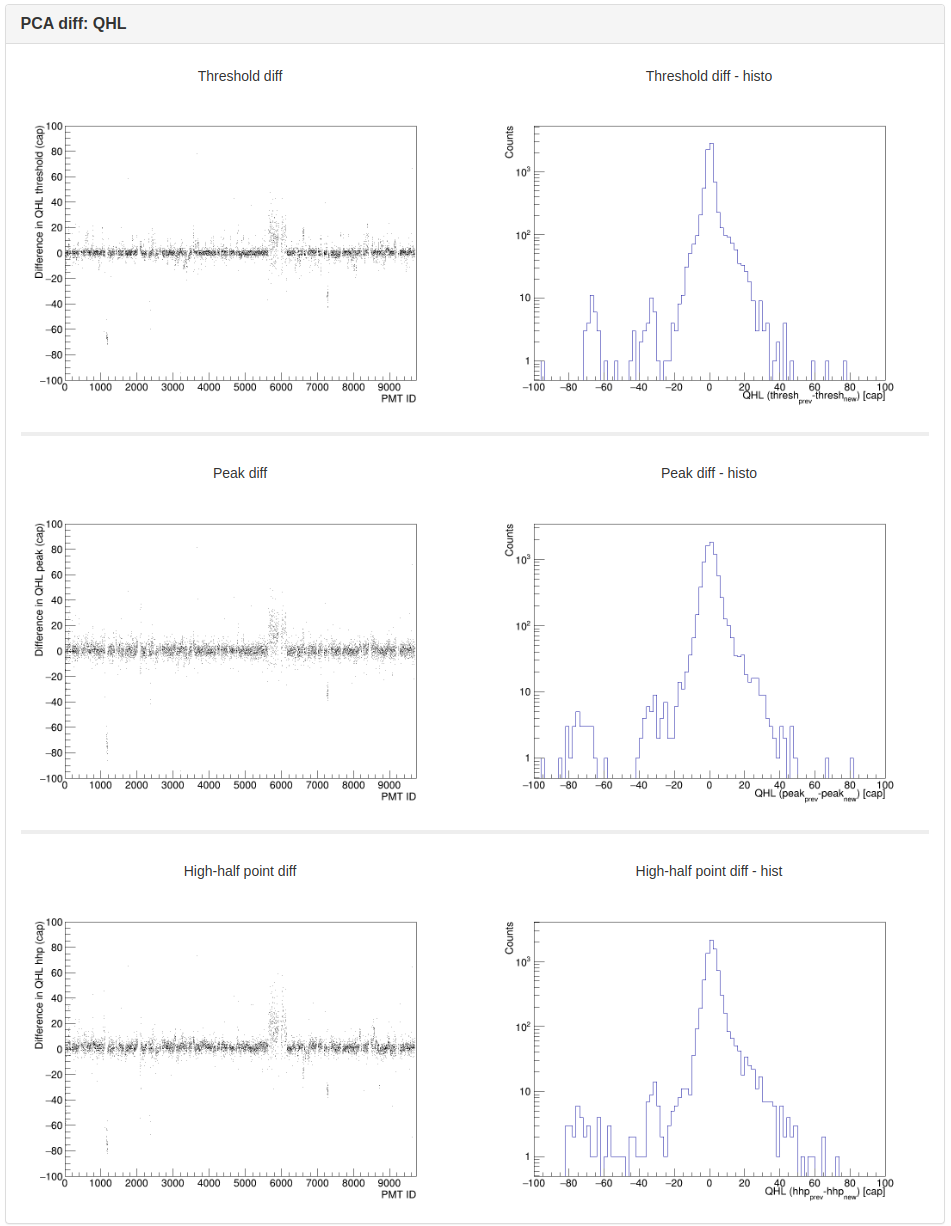
\includegraphics[width=1.1\textwidth]{./plots/pca6.png}}
  \caption{\centering \texttt{PCA Processor}: QHL charge data \#2.\hspace{\textwidth}This time showing the previously mentioned charge values as a difference of newly measured and latest value.}
  \label{fig:pca6}
\end{figure}

\begin{figure}
\centering
\noindent\makebox[1\textwidth]{
  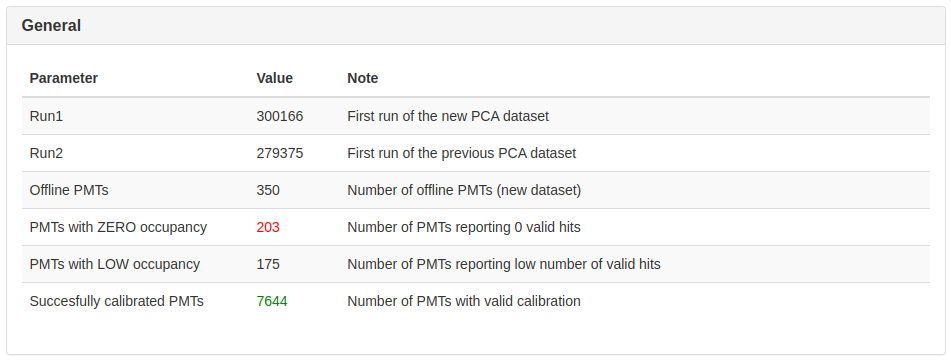
\includegraphics[width=1.1\textwidth]{./plots/bench1.png}}
  \caption{\centering \texttt{Benchmarking}: General section.\hspace{\textwidth}This summarizes basic benchmarking data such as: run numbers (starting number of the set), \# of offline PMTs for each set, PMTs with zero and low occupancy, and successfully calibrated PMTs.}
  \label{fig:bench1}
\end{figure}

\begin{figure}
\centering
\noindent\makebox[1\textwidth]{
  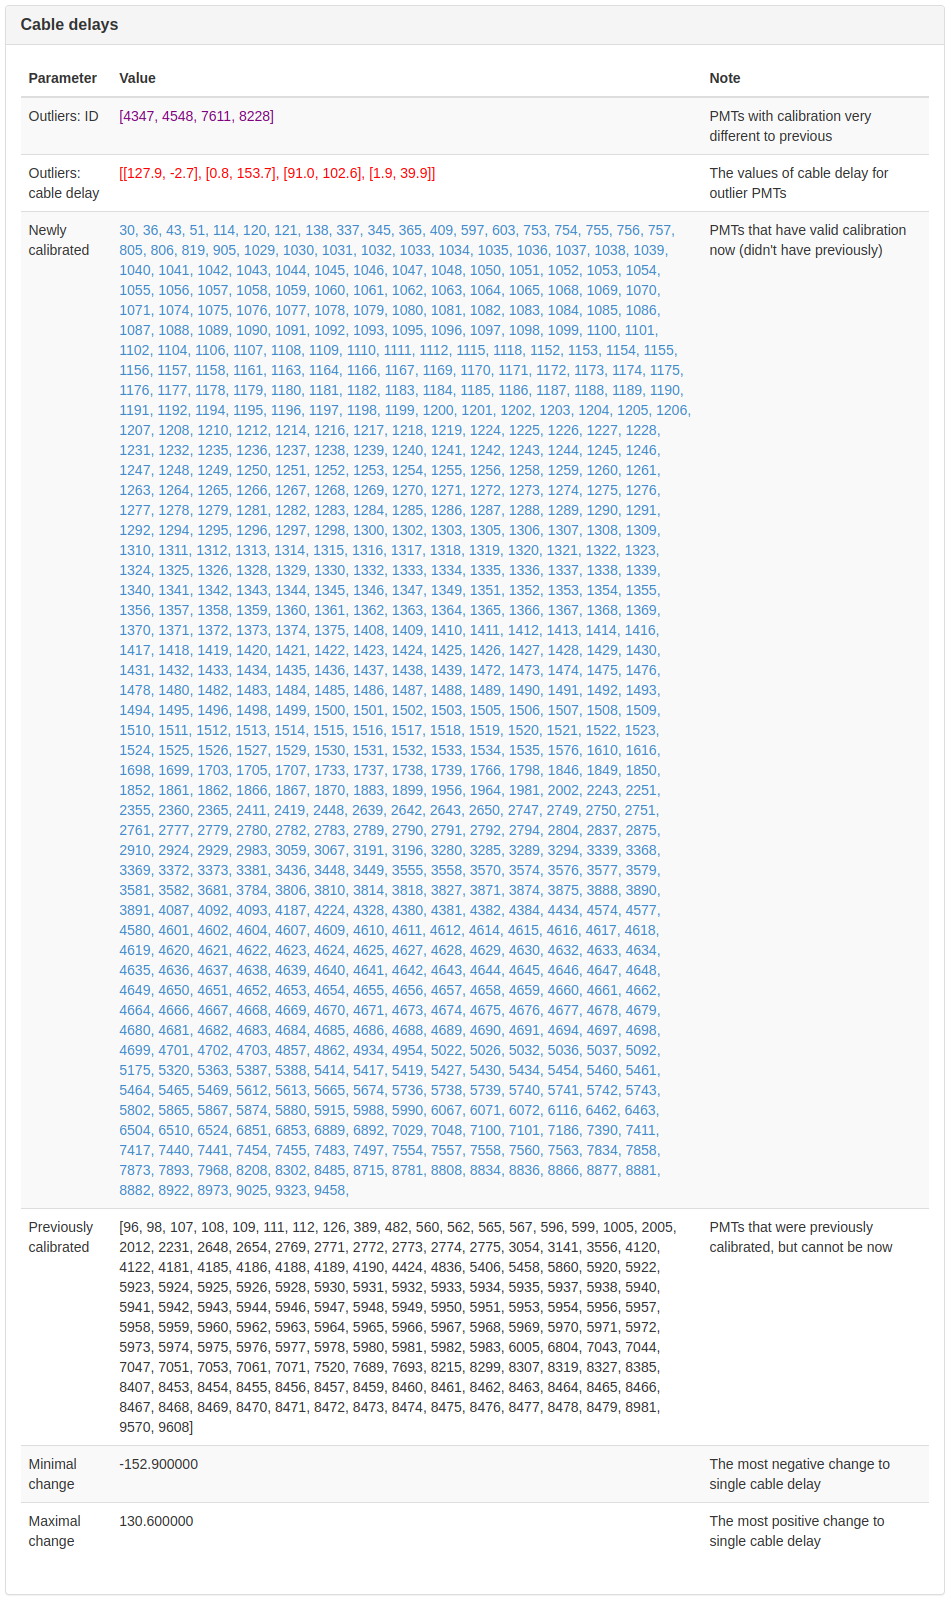
\includegraphics[width=0.81\textwidth]{./plots/bench2.png}}
  \caption{\centering \texttt{Benchmarking}: Cable delays data.\hspace{\textwidth}This section shows cable delays data for PMTs. Outliers are PMTs with new cable delay value very different to previous. PMTs that are now calibrated that were not before are shown (can be clicked, showing the actual PMT data), as well as PMTs that were previously calibrated but couldn't be in this set.}
  \label{fig:bench2}
\end{figure}

\begin{figure}
\centering
\noindent\makebox[1\textwidth]{
  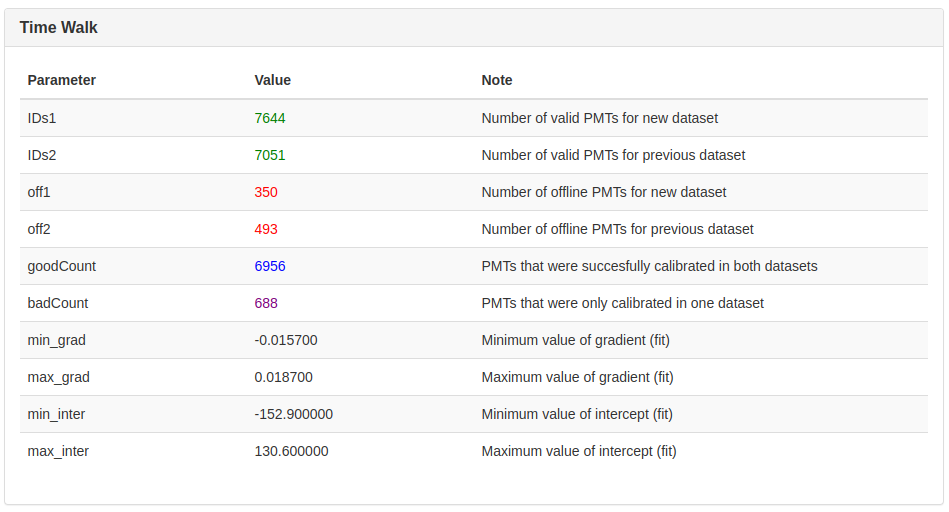
\includegraphics[width=1.1\textwidth]{./plots/bench3.png}}
  \caption{\centering \texttt{Benchmarking}: Time-walk data.\hspace{\textwidth}This is hopefully self-explanatory (see notes in the table).}
  \label{fig:bench3}
\end{figure}

\begin{figure}
\centering
\noindent\makebox[1\textwidth]{
  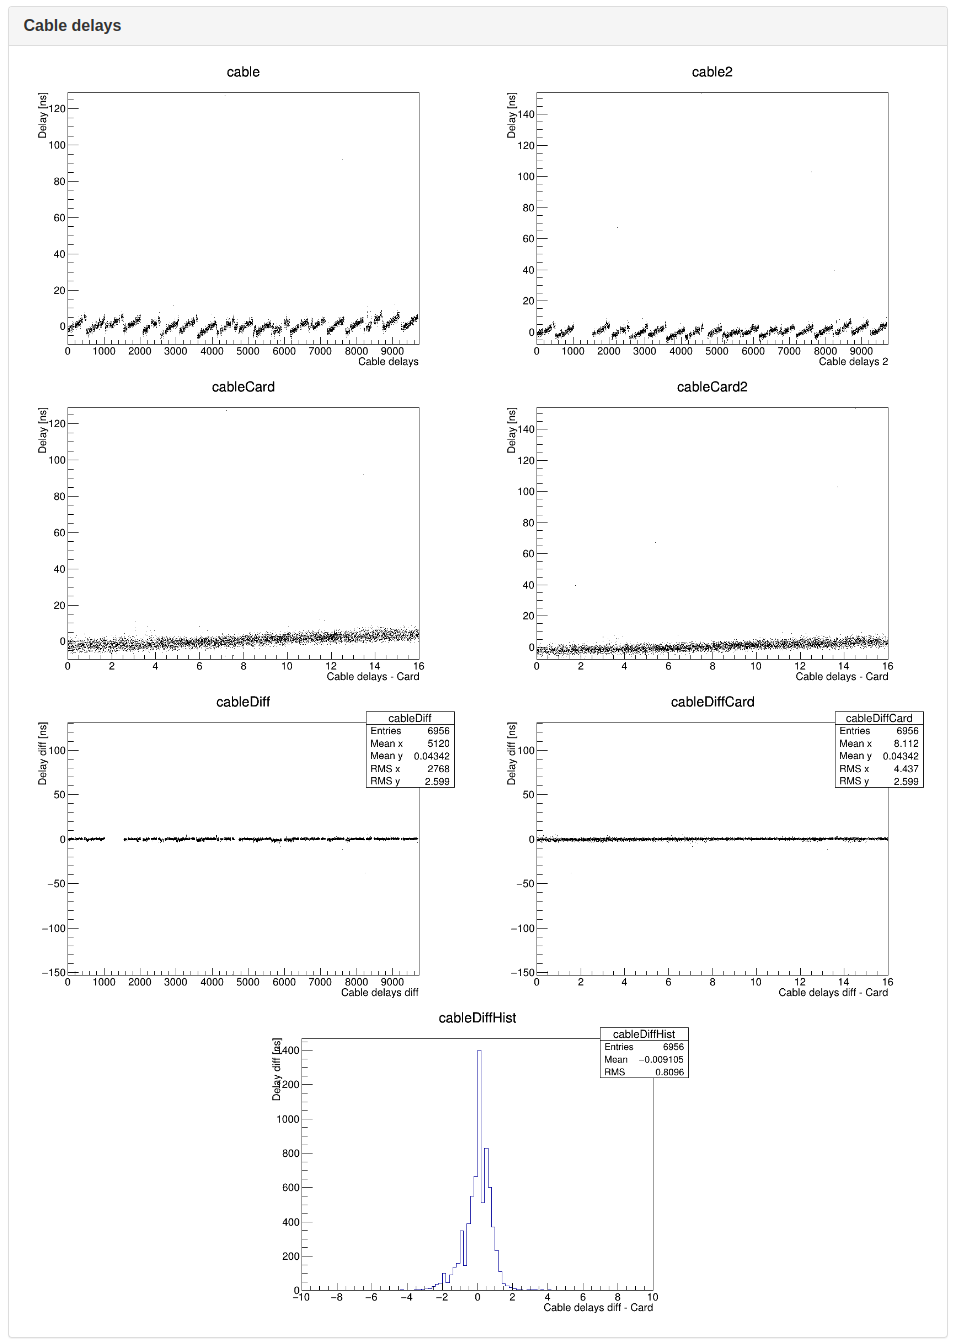
\includegraphics[width=0.95\textwidth]{./plots/bench4.png}}
  \caption{\centering \texttt{Benchmarking}: Plots for cable delays.\hspace{\textwidth}Showing the cable delays for this (left) and previous (right) calibration. Difference at the bottom.}
  \label{fig:bench4}
\end{figure}

\begin{figure}
\centering
\noindent\makebox[1\textwidth]{
  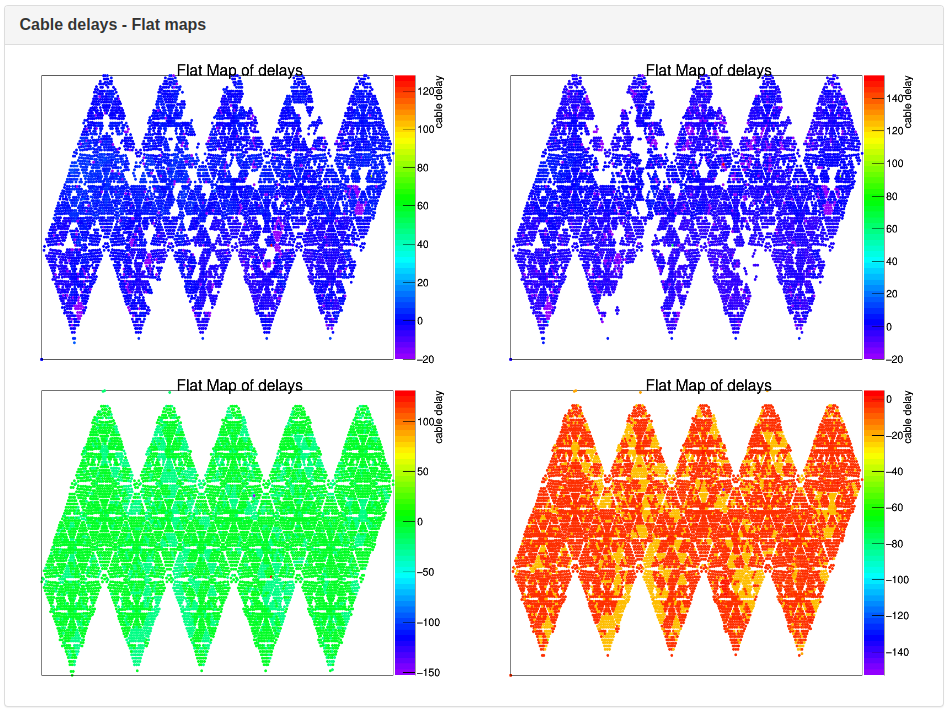
\includegraphics[width=1.1\textwidth]{./plots/bench5.png}}
  \caption{\centering \texttt{Benchmarking}: Flat map plots.\hspace{\textwidth}Top: flat maps showing the cable delays for this (left) and previous (right) set. Bottom: the difference of the cable delays between this and previous set (left); zoomed view of left plot (right).}
  \label{fig:bench5}
\end{figure}

\begin{figure}
\centering
\noindent\makebox[1\textwidth]{
  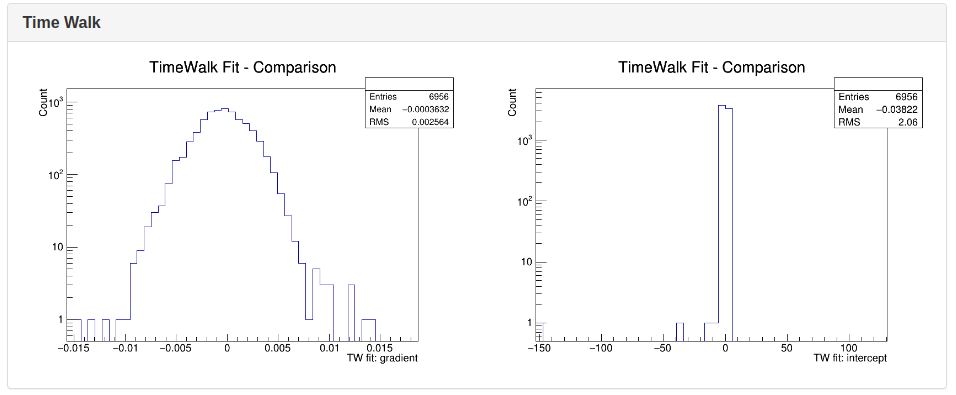
\includegraphics[width=1.1\textwidth]{./plots/bench6.png}}
  \caption{\centering \texttt{Benchmarking}: Time-walk plots.\hspace{\textwidth}The difference between this and previous set: TW gradient (left) and TW intercept (right).}
  \label{fig:bench6}
\end{figure}

\begin{figure}
\centering
\noindent\makebox[1\textwidth]{
  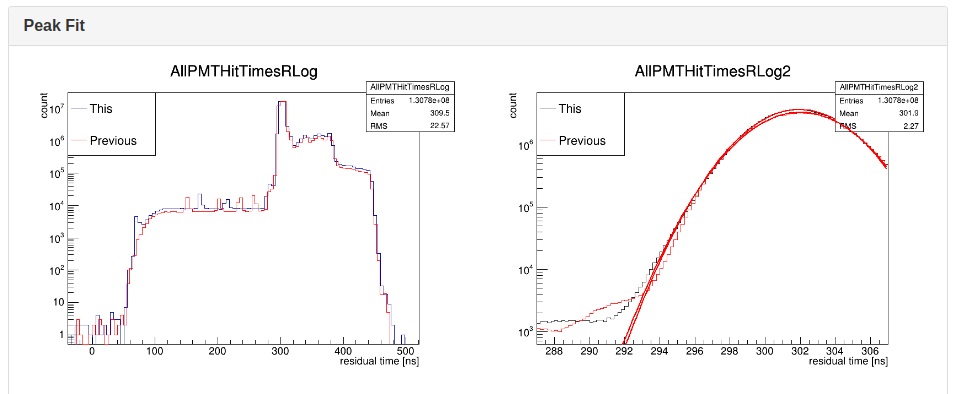
\includegraphics[width=1.1\textwidth]{./plots/bench7.png}}
  \caption{\centering \texttt{Benchmarking}: Peak fit plots.\hspace{\textwidth}These plots shown the residual hit times from a test laserball run, with the newly obtained, and old (previous set) cable delays applied to the PMT timings, respectively. Due to the difference of the actual number of PMTs that were calibrated, there will be difference. What is important is to look at the peak of this distribution (right plot).}
  \label{fig:bench7}
\end{figure}

\begin{figure}
\centering
\noindent\makebox[1\textwidth]{
  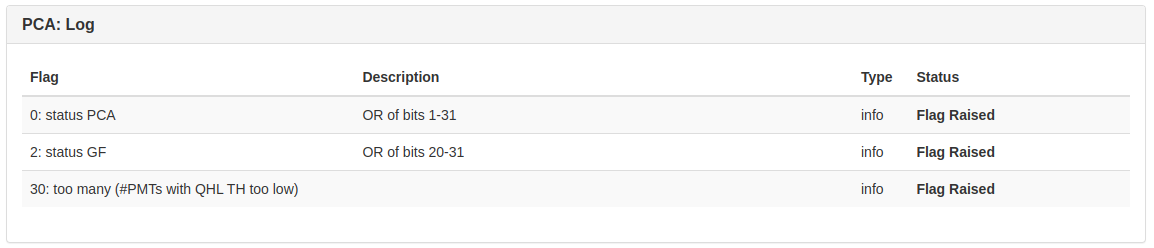
\includegraphics[width=1.1\textwidth]{./plots/log0.png}}
  \caption{\centering \texttt{Validation \#2}: \hspace{\textwidth}}
  \label{fig:log0}
\end{figure}

\begin{figure}
\centering
\noindent\makebox[1\textwidth]{
  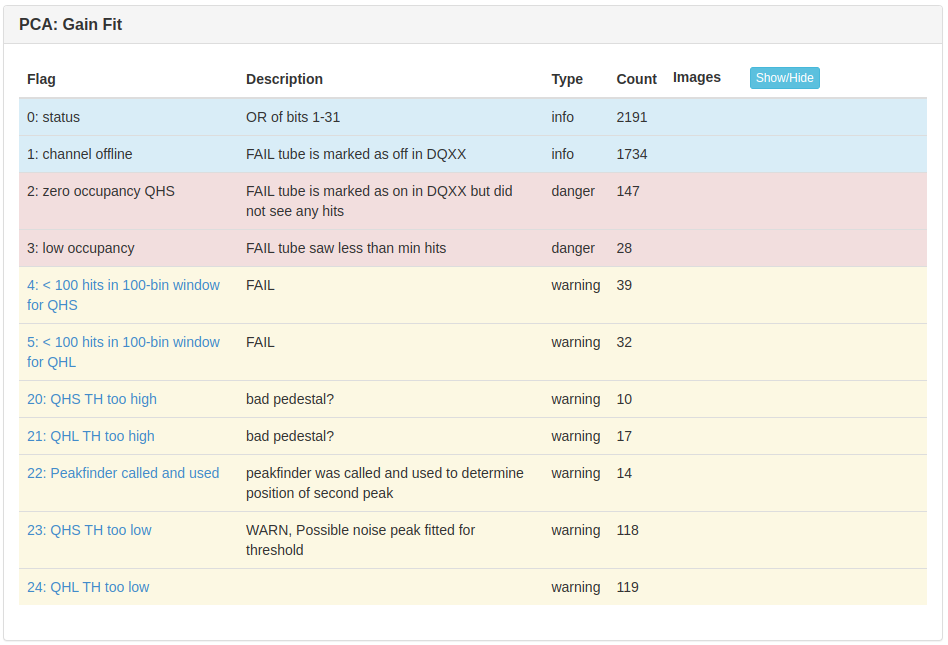
\includegraphics[width=1.1\textwidth]{./plots/log_gf.png}}
  \caption{\centering \texttt{Validation \#2}: \hspace{\textwidth}}
  \label{fig:log_gf}
\end{figure}

\begin{figure}
\centering
\noindent\makebox[1\textwidth]{
  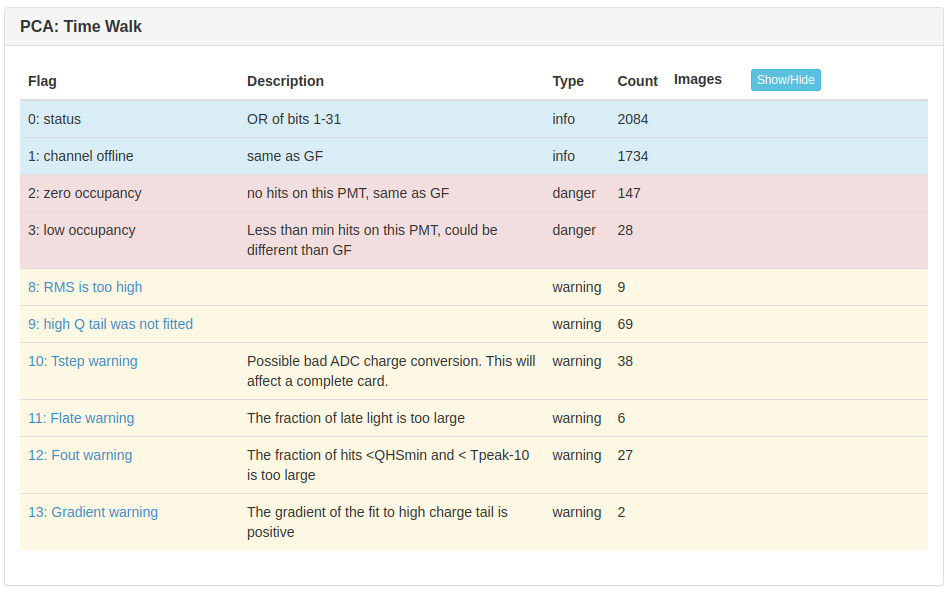
\includegraphics[width=1.1\textwidth]{./plots/log_tw.png}}
  \caption{\centering \texttt{Validation \#2}: \hspace{\textwidth}}
  \label{fig:log_tw}
\end{figure}

\begin{figure}
\centering
\noindent\makebox[1\textwidth]{
  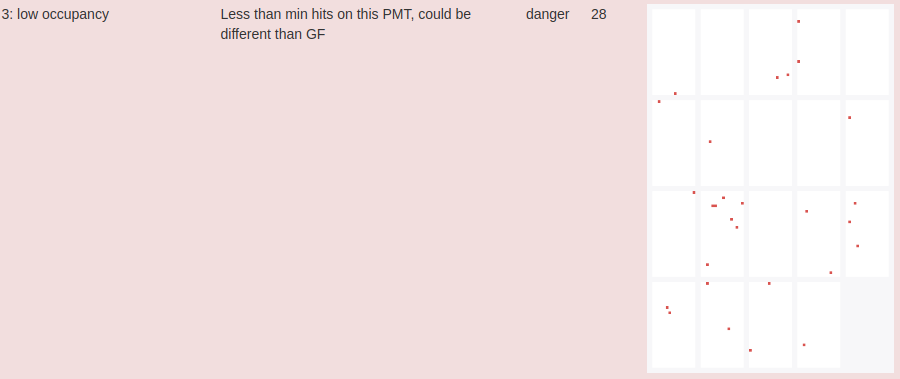
\includegraphics[width=1.1\textwidth]{./plots/log1.png}}
  \caption{\centering \texttt{Validation \#2}: \hspace{\textwidth}}
  \label{fig:log1}
\end{figure}

\begin{figure}
\centering
\noindent\makebox[1\textwidth]{
  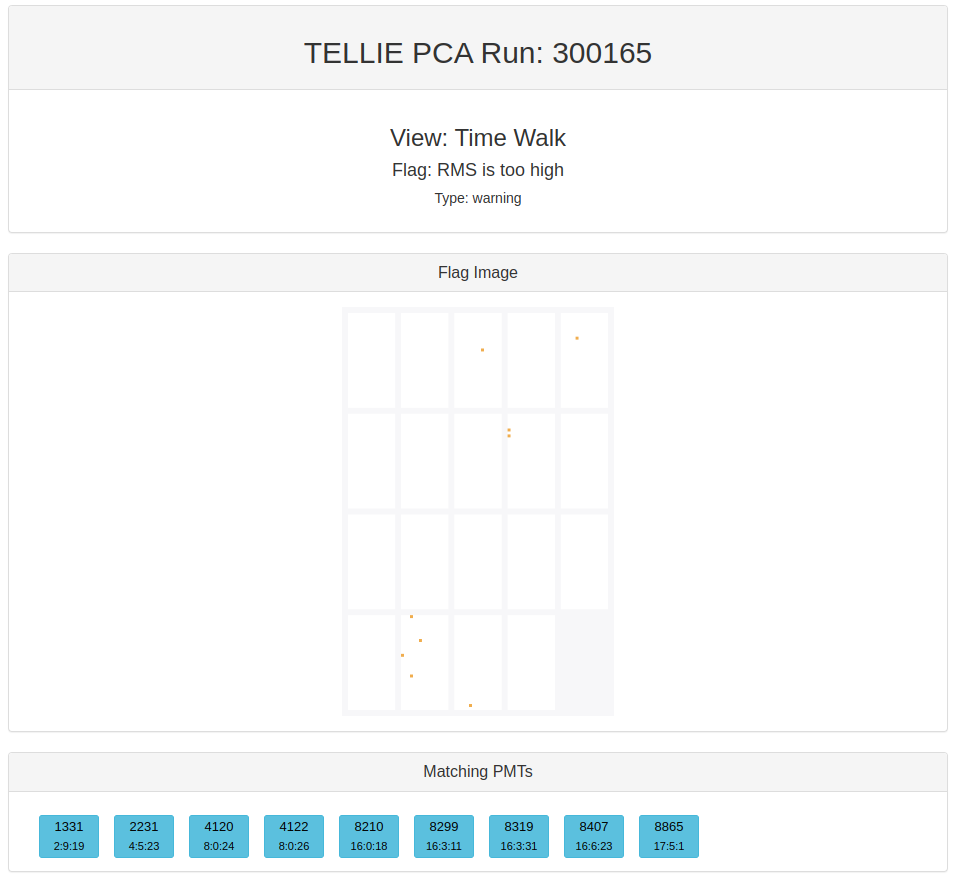
\includegraphics[width=1.1\textwidth]{./plots/log2.png}}
  \caption{\centering \texttt{Validation \#2}: \hspace{\textwidth}}
  \label{fig:log2}
\end{figure}

\begin{figure}
\centering
\noindent\makebox[1\textwidth]{
  \includegraphics[width=0.9\textwidth]{./plots/log3.png}}
  \caption{\centering \texttt{Validation \#2}: \hspace{\textwidth}}
  \label{fig:log3}
\end{figure}

\begin{figure}
\centering
\noindent\makebox[1\textwidth]{
  \includegraphics[width=1.1\textwidth]{./plots/min5.png}}
  \caption{\centering \texttt{Validation \#2}: \hspace{\textwidth}}
  \label{fig:min5}
\end{figure}

\begin{figure}
\centering
\noindent\makebox[1\textwidth]{
  \includegraphics[width=1.1\textwidth]{./plots/min6.png}}
  \caption{\centering \texttt{Validation \#2}: \hspace{\textwidth}}
  \label{fig:min6}
\end{figure}

\begin{figure}
\centering
\noindent\makebox[1\textwidth]{
  \includegraphics[width=1.1\textwidth]{./plots/min7.png}}
  \caption{\centering \texttt{Validation \#2}: \hspace{\textwidth}}
  \label{fig:min7}
\end{figure}

\begin{figure}
\centering
\noindent\makebox[1\textwidth]{
  \includegraphics[width=0.9\textwidth]{./plots/min9.png}}
  \caption{\centering \texttt{Validation \#2}: \hspace{\textwidth}}
  \label{fig:min9}
\end{figure}

\begin{figure}
\centering
\noindent\makebox[1\textwidth]{
  \includegraphics[width=0.9\textwidth]{./plots/min10.png}}
  \caption{\centering \texttt{Validation \#2}: \hspace{\textwidth}}
  \label{fig:min10}
\end{figure}

\begin{figure}
\centering
\noindent\makebox[1\textwidth]{
  \includegraphics[width=1.1\textwidth]{./plots/pmt1.png}}
  \caption{\centering \texttt{Validation \#2}: \hspace{\textwidth}}
  \label{fig:pmt1}
\end{figure}

\begin{figure}
\centering
\noindent\makebox[1\textwidth]{
  \includegraphics[width=1.1\textwidth]{./plots/pmt2.png}}
  \caption{\centering \texttt{Validation \#2}: \hspace{\textwidth}}
  \label{fig:pmt2}
\end{figure}

\clearpage

\section{System}
\paragraph{}
This section will describe some of the features of the overall processing.

\subsection{Simple}
\paragraph{}
The system is based on being very simple and with minimum human input. As it stands, it only needs to be started, providing a single text file with runs corresponding to a dataset.\\
Example runlist text file:
\begin{lstlisting}
300165
300167
300372
300171
300173
...
\end{lstlisting}

\subsection{Modular}
\paragraph{}
The whole system is a network of multiple individual steps, managed by one master script. The master script spawns subprocessed. Individual steps can be (re)run. Modules can be easily modified, separately.

\subsection{Submission platform}
\paragraph{}
To process the whole dataset, many individual jobs need to be run. There are 6 steps for each run: \texttt{Validation \#1}, \texttt{position fit}, \texttt{angular systematic fit}, \texttt{injection fit}; and addition steps to be run per dataset: \texttt{PCA Processor}. There are several other global jobs: creating PCA table, comparing PCA tables, checking PCA output, comparing time-walk data, benchmarking (multiple steps), final compare scripts (multiple). For a single set of 95 runs (one per fibre), this ends up totalling close to 600 (95*6 + global + other) individual processes.

\paragraph{}
To deal with this, the master scripts has inbuilt submission platform. It spaws child processes (up to a configurable limit) and monitors their status. There is a queue that holds jobs to be submitted. The whole system is run in steps, as usually consecutive steps require the output of previous steps. 

\paragraph{}
If processes fail, they are retried up to a limit. After that, the failed processes need to be investiaged and rerun manually (if needed).

\subsection{Customizable}
\paragraph{}
The checks in validation steps are often based on threshold values. There are loaded from environment and should be tuned before running. There are comments explaining what the threshold values are, please see Figure~\ref{fig:thresh}.

\begin{figure}
\centering
\noindent\makebox[1\textwidth]{
  \includegraphics[width=1.1\textwidth]{./plots/thresh.png}}
  \caption{\centering The threshold parameters, used for validation. These can be tuned as required.}
  \label{fig:thresh}
\end{figure}

\subsection{Linked}
\paragraph{}
The processing system is linked to multiple databases. The CouchDB holds data on: belly plates, benchmarking, environment constants, list of fibres, runlists, and document for each run/fit combination. An overview of views in the couhdb is shown in Figure~\ref{fig:couch}, while an example environment CouchDB document is shown in Figure~\ref{fig:couchdoc}.

\begin{figure}
\centering
\noindent\makebox[1\textwidth]{
  \includegraphics[width=0.5\textwidth]{./plots/couch.png}}
  \caption{\centering \texttt{Validation \#2}: }
  \label{fig:couch}
\end{figure}

\begin{figure}
\centering
\noindent\makebox[1\textwidth]{
  \includegraphics[width=0.32\textwidth]{./plots/couchdoc.png}}
  \caption{\centering \texttt{Validation \#2}:  }
  \label{fig:couchdoc}
\end{figure}

\paragraph{}
Additionally, the system requires access to ratDB. Finally, there is a plethora of plots created. These need to be linked to minard, usually via nfs mount over network.

\subsection{Regulation}
\paragraph{}
The system was developped to have unified cuts, event selection, checks, and ranges.

\subsection{Evaluative}
\paragraph{}
There are bitwords used in \texttt{Validation \#1} and \texttt{Validation \#2}. There are a proxy for the quality of the data. If tuned correctly, these could be used to ignore specific runs, however, this is not currently implemented.

\clearpage

\section{Code}
\subsection{Master scripts}

\section{Deploying}

\section{Running}

\section{ToDos}

\section{Other documentation}


\end{document}
